\section{Hardwareentwicklung, Softwarebackend \\ und Benutzeroberfläche \textcolor{gray}{(Benedikt Simbürger)}}

\subsection{Hardware}

\subsubsection{Planung - Grundanforderungen} 
Grundlegende Anforderungen zur Planung der AFSS-Mechanik sind Transportfähigkeit, eine möglichst einfache Realisierung mit HTL-Mitteln und möglichst wenige Kompromisse in der Funktion oder Zuverlässigkeit eingehen zu müssen.\\
Die Anforderung der Transportfähigkeit limitiert die Größe des Lagers auf \SI{2.3}{\meter} Länge, um im Lift transportiert werden zu können, und auf \SI{1.9}{\meter} Höhe aufgrund der Türhöhe im Keller. Weiters müssen auch noch Rollen an den Rahmen angebracht werden, um das Lager ohne großen Mehraufwand bewegen zu können. Diese Extrahöhe der Räder (ca. \SI{80}{\mm}) limitiert den Rahmen weiter.\\
Nun soll dieser rund \SI{2.25}{\meter} lange und \SI{1.8}{\meter} hohe Raum optimal genutzt werden, um eine möglichst große Lagerdichte sicherstellen zu können.\\
Um eine möglichst gute Erweiterbarkeit sowie eine Fertigung an der Schule zu ermöglichen, sollen für die mechanische Trägerkonstruktion sogenannte Item-Profile verwendet werden.



\paragraph{Item}\mbox{}\\
Das Item-Profilsystem ist ein System, welches Aluminium-Extrusionen in verschiedenen Ausführungen sowie viele Verbindungsmöglichkeiten zu sich selbst sowie anderen mechanischen Elementen bietet. Hierbei gibt es eine breite Auswahl an Profilen, von 20x20 mm bis 40x40 mm Querschnitt. Für alle Komponenten mit hoher mechanischer Beanspruchung werden 40x40-Extrusionen verbaut, da diese eine besonders hohe Biegefestigkeit aufweisen. Für Anwendungen mit geringerer Beanspruchung sowie aus Platz- und Gewichtsparmaßnahmen werden 20x20-Extrusionen verwendet.
Zur Verbindung zu anderen Bauelementen gibt es die Möglichkeit, Nutensteine mit verschiedenen Gewinden in die Nut einzulegen und dort Platten o. Ä. anzuschrauben. Um Item-Profile untereinander zu verbinden, können Standardverbindungssätze wie in Abb. \ref{sfs_item} verwendet werden.\\

Die Anwendung im AFSS erfordert ausserdem recht lange Verfahrwege. Um dies kostengünstig umsetzen zu können, werden V-Slot-Profile verwendet.

\begin{figure}[H]
    \begin{minipage}{0.5\textwidth}
        \centering
        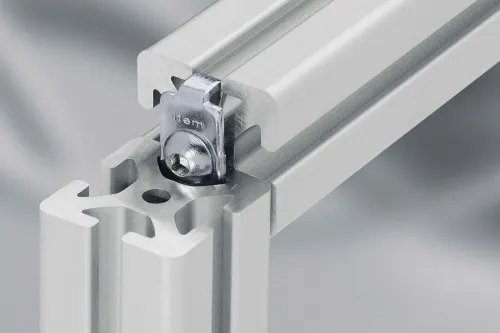
\includegraphics[width=0.9\textwidth]{Item-Standartverbindungssatz.png}
        \caption{Item Profil mit Standartverbindungssatz, Quelle: \cite{Item_svs}}
        \label{sfs_item}
    \end{minipage}%
    \begin{minipage}{0.5\textwidth}
        \centering
        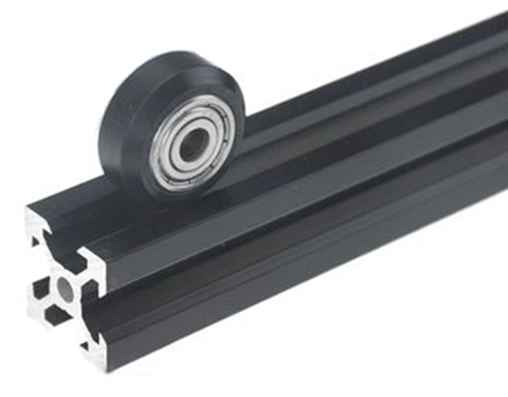
\includegraphics[width=0.9\textwidth]{V-Wheel.jpg}
        \caption{V-Slot-Profil mit V-Wheel, Quelle: \cite{v_slot_wheel}}
        \label{v-wheel}
    \end{minipage}
\end{figure}


\paragraph{V-Slot}\mbox{}\\
Auch V-Slot-Profile sind Aluminium-Extrusionen. Diese können grundsätzlich auch ähnlich wie Item-Profile mit Nutensteinen etc. verwendet werden, sind aber zusätzlich darauf ausgelegt, dass ein V-Wheel in einer Narbe des Profils rollen kann (siehe Abb. \ref{v-wheel}). Diese Profile sind in einer C-Profil-Form erhältlich. Diese sind für die langen Verfahrwege optimal, da einerseits auch breitere und mehr V-Wheels verwendet werden können, sowie einen sehr großen Widerstandsmoment aufweisen.


\subsubsection{Vorgehensweise}
Aufgrund der besonderen und sehr komplexen Anforderungen dieser Mechanik erfolgt die Entwicklung in mehreren Iterationen. Nach Auslegung der Grundparameter wird eine Grundkonstruktion erstellt, um mögliche Lösungsansätze für die jeweiligen Komponenten zu skizzieren. Durch diese grobe Planung können viele Konzepte mit geringerem Zeitaufwand iteriert werden und auch mögliche Missverständnisse o. Ä. frühzeitig aufgeklärt und überarbeitet werden. Weiters werden bei diesem Prozess wichtige Fähigkeiten in der Bedienung der CAD-Software gewonnen und so die Geschwindigkeit der zukünftigen Designiterationen beschleunigt.\\
Um bestimmte Elemente der Mechanik einzeln zu testen, werden auch mehrere Prototypen gebaut und die gewonnenen Erkenntnisse in die finale Konstruktion miteingebunden.\\

\begin{figure}[H]
    \centering
    \begin{subfigure}{.3\textwidth}
        \centering
        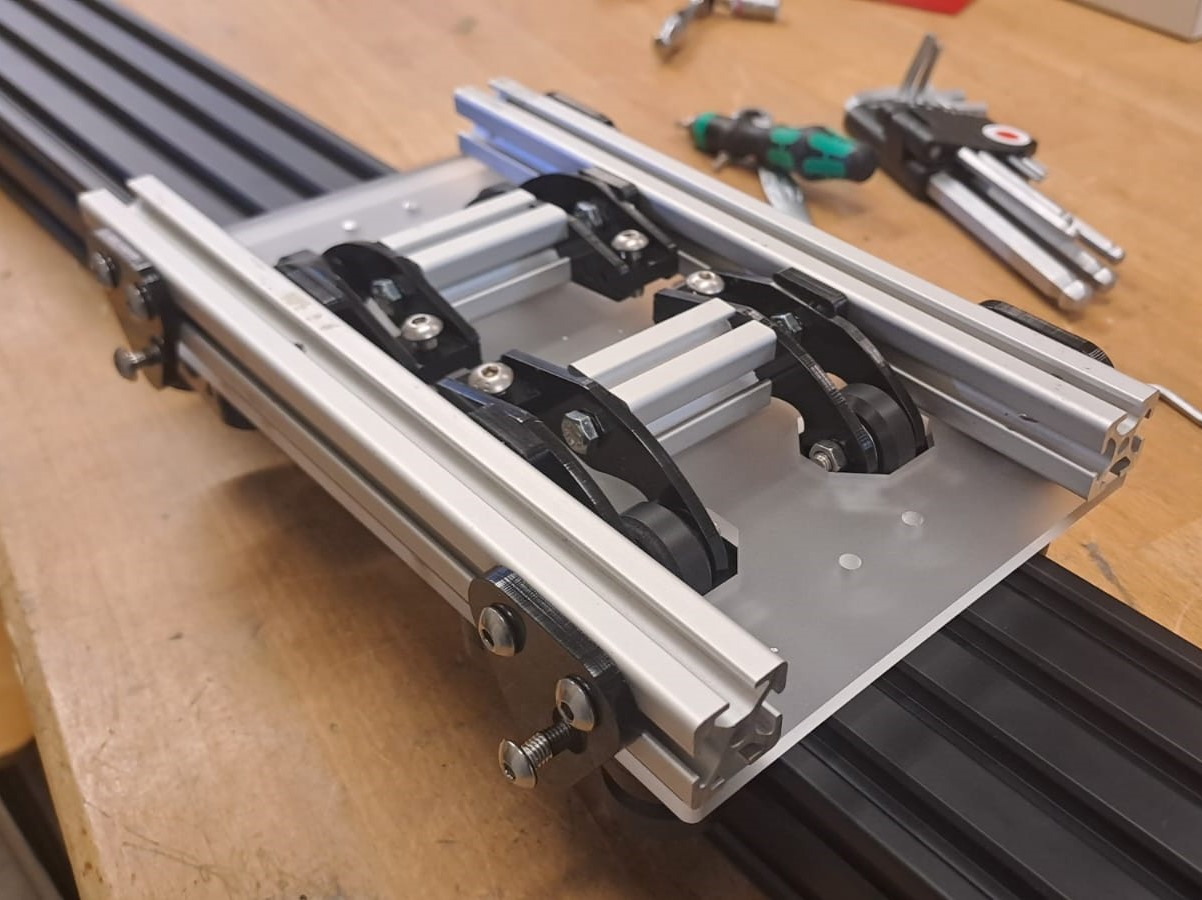
\includegraphics[width=0.9\textwidth]{pt_x.jpg}
        \caption{X-Achse}
        \label{pts:plt_x}
    \end{subfigure}%
    \begin{subfigure}{.3\textwidth}
        \centering
        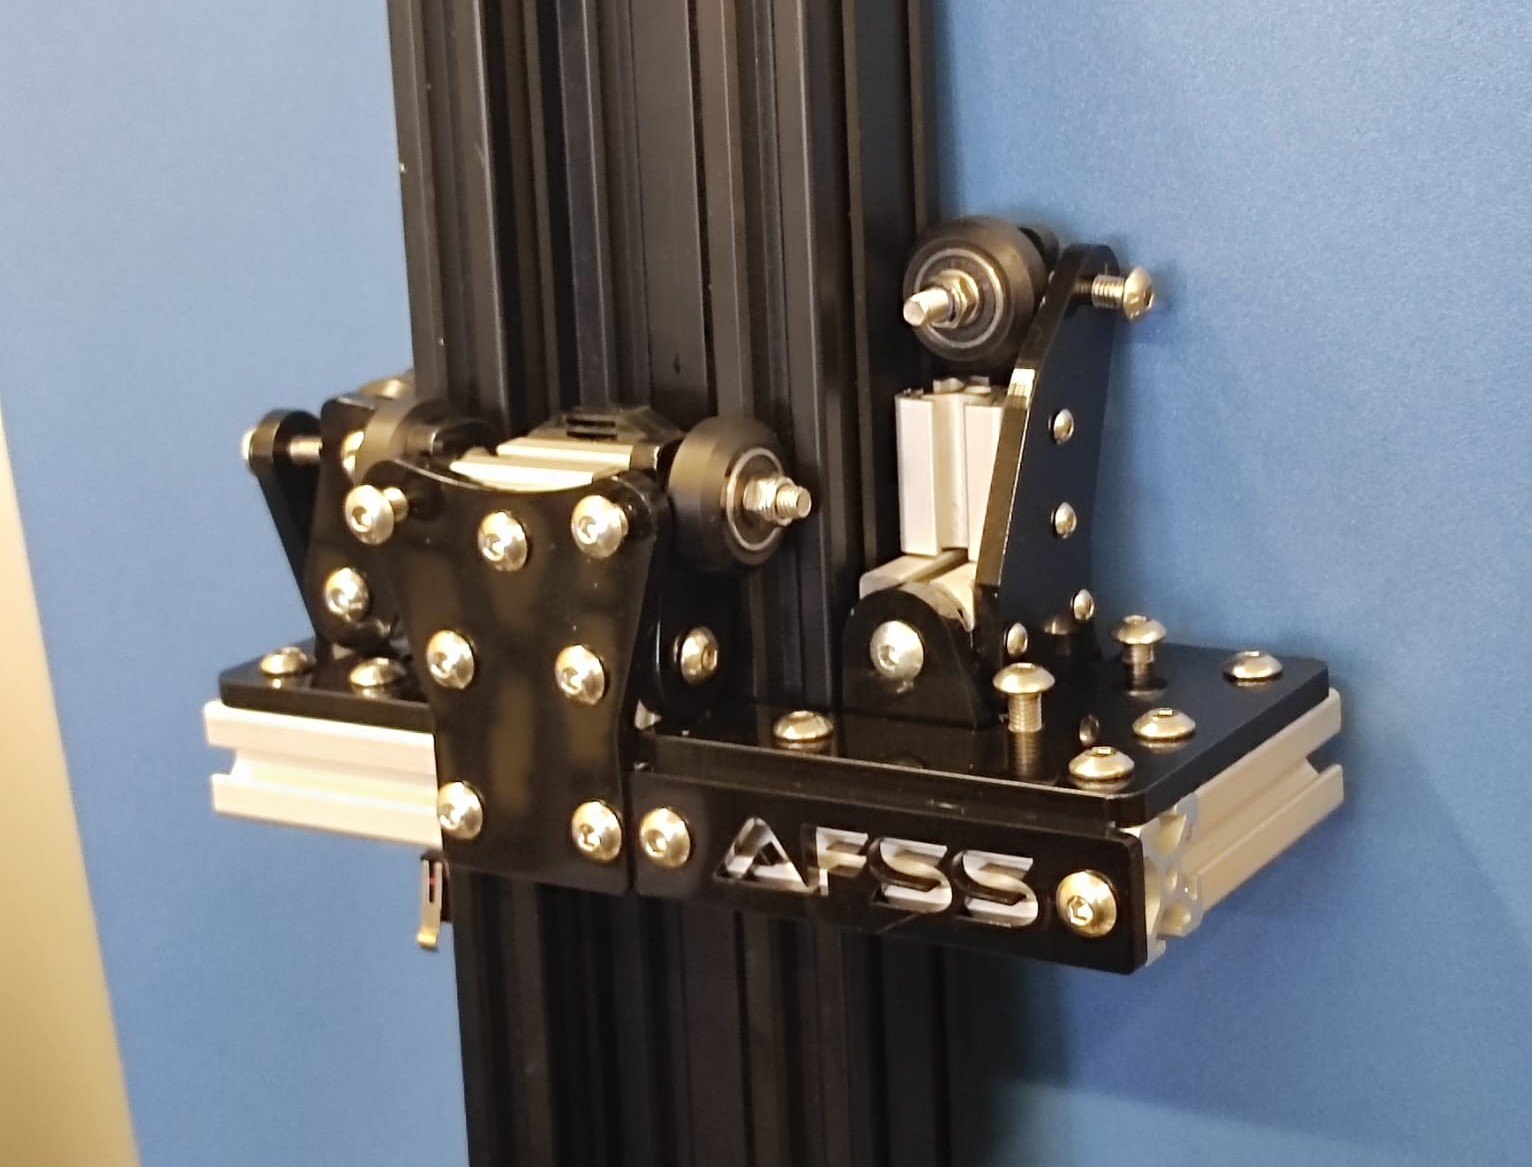
\includegraphics[width=0.9\textwidth]{pt_y.jpg}
        \caption{Y-Achse}
        \label{pts:plt_y}
    \end{subfigure}%
    \begin{subfigure}{.3\textwidth}
        \centering
        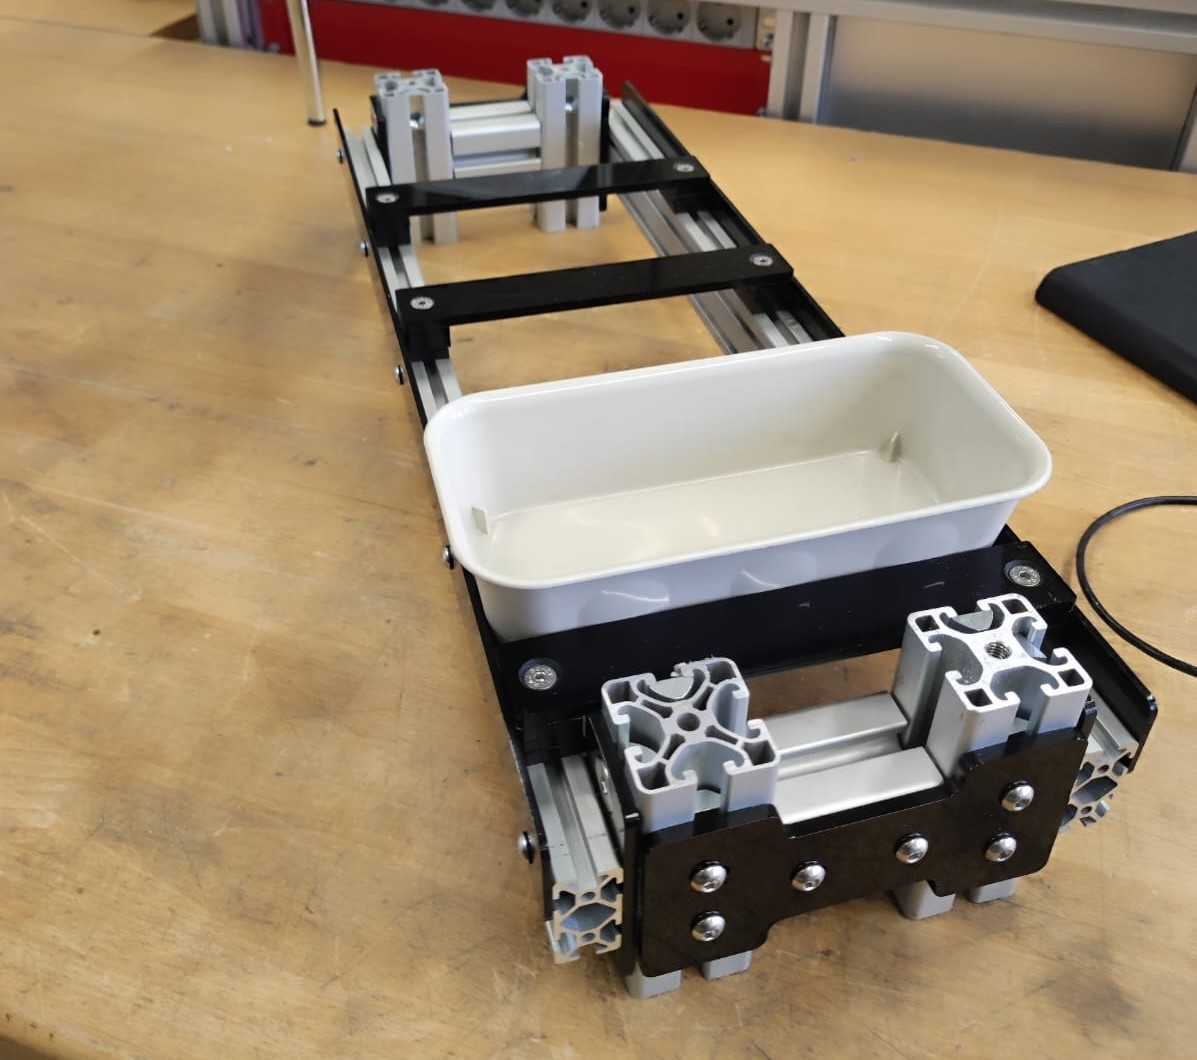
\includegraphics[width=0.9\textwidth]{pt_lg.jpg}
        \caption{Lagerregal}
        \label{pts:plt_ls}
    \end{subfigure}
    \caption{Prototypen}
    \label{pts}
\end{figure}
\vspace{-3mm}

\paragraph{Rahmenbedingungen für die Fertigung}\mbox{}\\
Damit die Fertigung der Mechanik an der HTL-Mössingerstraße in einem realistischen Zeitrahmen möglich ist, müssen gewisse Rahmenbedingungen bei der Planung beachtet werden.
\begin{itemize}
    \item Für Verbindungen mit geringer bis mittlerer mechanischer Beanspruchung werden Bauteile so geplant, dass diese im Lasercutter gefertigt werden können, sowie in den Stärken, die der Werkstätte zur Verfügung stehen (\qtylist{3;4;5}{\milli\meter}). Dabei muss beachtet werden, dass die Acrylplatten gegossen sind und dadurch recht hohe Toleranzen (bis zu +\SI{0.3}{\milli\meter}) aufweisen.
    \item Verbindungen zwischen Platten und Item- oder V-Slot-Profilen werden möglichst einheitlich gestaltet. Grundsätzlich gilt: Verbindungen mit Item-Baureihe BR5 (20x20) werden grundsätzlich in M5 ausgeführt, außer bei Platzmangel in M3. Verbindungen mit BR 8 (40x40) werden in M8 ausgeführt.
    \item Bei Bauteilen mit hoher mechanischer Beanspruchung wird Aluminiumblech mit 5 mm Stärke verwendet. Dieses wird zwar CNC-gefräst, doch um bei der Fertigung Zeit zu sparen, wird davon abgesehen, Taschen o. Ä. einzuplanen. Stattdessen wird immer ein flaches Profil verwendet, welches sich mit 2.5D-Fräsverfahren mit Durchgangsfräsen, ähnlich einem Lasercutter, fertigen lässt. Bei Aluminiumteilen wird darauf geachtet, dass diese immer aus \SI{5}{\mm} dickem Aluminiumeloxal gefertigt werden.
\end{itemize}



\paragraph{Konstruktionsvorgang}\mbox{}\\
Um ein so umfangreiches Projekt umsetzen zu können, muss auch bei der 3D-Planung größtmögliche Ordnung herrschen. Um effizient zu arbeiten, werden wiederverwendbare Bauteile in einer eigens angelegten Bauteilbibliothek abgelegt. So können beispielsweise Aluminiumprofile in Normlängen oder Sensoren einfach in die aktuelle Konstruktion eingefügt werden, ohne diese jedes Mal neu konstruieren zu müssen.
\\
Auch innerhalb einer Konstruktion ist auf Übersichtlichkeit zu achten. Zu diesem Zweck ist es sinnvoll, zusammenhängende Objekte in Komponenten zusammenzufassen. Diese sind vergleichbar mit Ordnern. Wie auch Ordner können Komponenten ineinander verschachtelt werden. Dadurch lässt sich eine saubere Struktur umsetzen, die es beispielsweise erleichtert, einzelne Konstruktionsteile zu betrachten oder gezielt Änderungen daran vorzunehmen.


\subsubsection{Rahmen}

Der Rahmen des AFSS bezeichnet jene Struktur, die sowohl als äußeres Gehäuse als auch zur grundlegenden mechanischen Stabilität dient. Er soll die maximal zulässige Höhe und Länge optimal ausnutzen, während die Breite so gering wie möglich gehalten wird.
\\
Umgesetzt wird dies mit einem Gerüst aus 40x40-Aluminium-Extrusionen. Dieses besitzt zusätzlich oben und unten zwei Längsstreben, die eine möglichst platzsparende Aufhängung der X-Achsen-V-Slot-Profile ermöglichen. Auf einer Seite wird zudem eine Aussparung eingeplant, um ausreichend Freiraum zu schaffen, damit der Querförderer die Boxen reibungslos auf das Förderband transportieren kann.
\\
Weiterhin muss berücksichtigt werden, dass Rollen für den Transport angebracht werden. Da diese die maximale Höhe beeinflussen, muss dies in die Planung der Y-Achse einfließen, um sicherzustellen, dass das System problemlos durch Türen bewegt werden kann.

\subsubsection{X-Achse}
Die X-Achse des AFSS ist das mechanische Herzstück. Sie ist die Achse, die sich horizontal bewegt und einen langen Verfahrweg sowie hohe mechanische Anforderungen besitzt. Sie muss sowohl ihr Eigengewicht als auch das Gewicht der YZ-Achse tragen.
\\
Das Grundelement der X-Achse besteht aus V-Slot-C-Profilen, die oben und unten aufgehängt werden. Diese Profile sind in Längen von \SI{1.5}{\meter} erhältlich, daher wird die gesamte Achse so ausgelegt, dass zwei Stück (also insgesamt \SI{3}{\meter} Schiene) verwendet werden. Zusätzlich sind die Profile mit jeweils sechs Nivellierungsschrauben pro V-Profil ausgestattet, um sie möglichst parallel zueinander sowie exakt in Waage auszurichten.

\paragraph{Grundanforderungen}\mbox{}\\
Auf der X-Achse bewegt sich der X-Schlitten, dessen Aufgabe es ist, die Y-Achse präzise zu positionieren. Dafür muss er alle erforderlichen Motoren und Sensoren enthalten. Zudem muss er einen Angriffspunkt bieten, um seine Bewegung zu ermöglichen.
\\
Der Schlitten sollte sowohl horizontal als auch vertikal möglichst kompakt konstruiert sein, um einen maximalen Verfahrweg in X- und Y-Richtung zu gewährleisten.

\paragraph{Antrieb}\mbox{}\\
Angetrieben wird die X-Achse mit zwei Schrittmotoren, welche jeweils an einer Schiene (oben und unten) angebracht werden. Diese treiben mithilfe eines Zahnriemens die zwei X-Schlitten an. Als Zahnriemen wurde aufgrund der hohen Kraftübertragung sowie der großen Länge ein AT5-Zahnprofil mit \SI{16}{\mm} Riemenbreite der Firma Mähdler gewählt. Dieser wird vom Motor über eine entsprechende Zahnscheibe angetrieben und am Shuttle befestigt. Als Schrittmotor wird aus Einfachheitsgründen dasselbe Modell wie bei der Y-Achse verwendet. Diese erzeugen auch genügend Moment, um die X-Achse anzutreiben.

\paragraph{Riemenspannung X-Achse} \mbox{}\\
Da der Riemen für eine zuverlässige Kraftübertragung bei so langen Verfahrwegen eine relativ große Vorspannkraft benötigt, ist das Zahnriemenklemmelement auf der X-Achse auch dementsprechend auszuführen. Um den Zahnriemen zu greifen, werden Teile mit Negativverzahnung 3D-gedruckt, in dieses der Zahnriemen dann auf beiden Seiten des Schlittens geklemmt wird. Die Aufhängung der einen Seite ist einfach mit den Item-Profilen verschraubt, lässt aber noch etwas Platz, um den Riemen mit der Hand vorzuspannen. Auf der anderen Seite ist das Klembrett über zwei Gewindestangen mit dem restlichen Shuttle verbunden. Diese können festgezogen werden, um die nötigen Vorspannkräfte zu erzeugen (siehe \ref{X-Achse_a1}). Außerdem ist diese Spannvorrichtung in einem Formfaktor ausgeführt, welcher es erlaubt, direkt darüber die Motoren der Y-Achse anzubringen (siehe \ref{X-Achse_a2}).

\paragraph{Achsenführung} \mbox{}\\
Die Führung der Achse im V-Slot-Profil wird mit V-Wheels durchgeführt. Sechs V-Wheels werden von oben auf das C-Profil gedrückt. Jedes Rad wird einzeln aufgehängt. Weiters ist überall eine Schraube verbaut, mit welcher das Rad weiter in die Führung hineingedrückt werden kann, sowie ein bis zwei Klemmpunkte, um bei Betrieb die Last von der Spannschraube nehmen zu können. Durch den geringen Platz im Schlitten ist es durchaus eine Herausforderung, dass all diese Mechanik neben den Spannelementen und Motoren in einem so kleinen Shuttle Platz finden. Auf der Seite des Schlittens werden noch weitere V-Wheels angebracht, welche die Spurführung übernehmen.
Im oberen Schlitten werden nur diese Führungsräder verbaut, da es nicht möglich und nötig ist, vertikale Kräfte zu unterstützen.

\paragraph{Kabelführung} \mbox{}\\
Um Sensoren und Aktoren der Y- und Z-Achse zu unterstützen, müssen dementsprechende Leitungen auf das X-Shuttle verlegt werden. Dies wird mithilfe einer Kabelschleppkette der Firma Igus umgesetzt. Diese wird parallel zum unteren C-Profil verlegt und unter Berücksichtigung der Biegeradien am X-Shuttle befestigt. Bei dieser ist darauf zu achten, dass sie alle benötigten Leitungen sowie genügend Freiraum für die Biegung einhält (vgl. \cite{igus_freitragend}). Weiters müssen Signal- und Aktorstromkreise durch Trennstege voneinander getrennt werden.
\\
Um die weiteren Geräte am AFSS zu versorgen, müssen zusätzlich noch Verdrahtungskanäle am Rahmen angebracht werden.

\paragraph{Sensoren}\mbox{}\\
Die Sensorik ist bei jeder Achse ähnlich aufgebaut. Immer zwei Endschalter und ein Referenzierschalter. Bei der X-Achse werden als Endschalter mechanische Rolltaster verwendet. Diese werden neben den V-Slot-Profilen befestigt und von einem, vom Schlitten abstreifenden Arm ausgelöst.


%zwei abbildungen nebeneinander mit legende
\begin{figure}[H]
    \centering
    \begin{subfigure}{.5\textwidth}
        \centering
        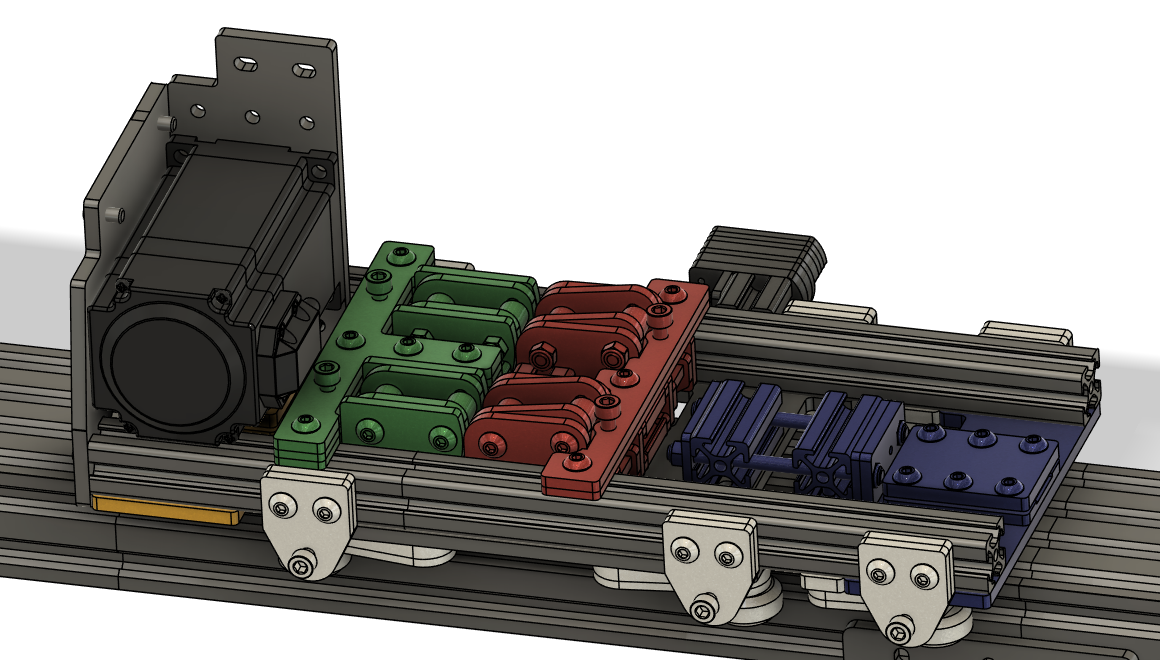
\includegraphics[width=0.94\textwidth]{X-Achse_a1.png}
        \caption{X-Schuttle Ansicht hinten\\ (Motor rechts und Rollen ausgeblendet)}
        \label{X-Achse_a1}
    \end{subfigure}%
    \begin{subfigure}{.5\textwidth}
        \centering
        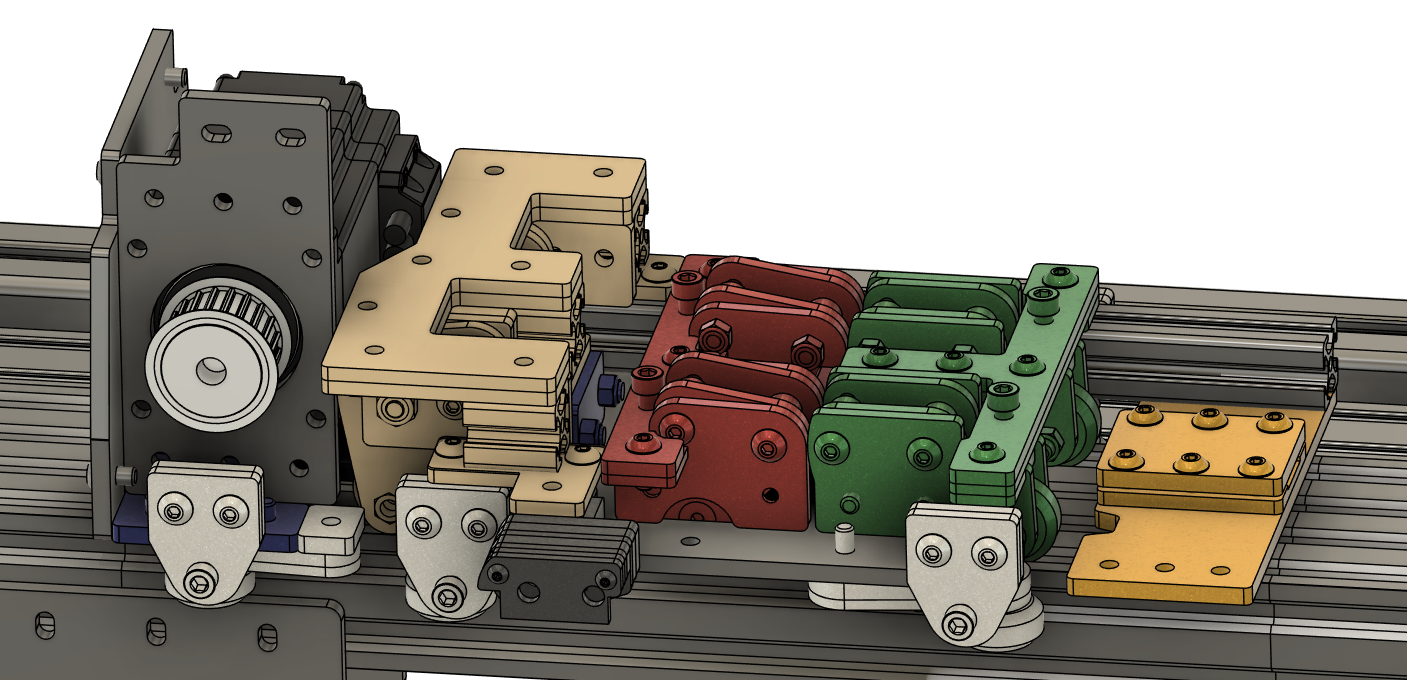
\includegraphics[width=0.94\textwidth]{X-Achse_a2.png}
        \caption{X-Schuttle Ansicht vorne \\(Motor rechts und Profil vorne ausgeblendet)}
        \label{X-Achse_a2}
    \end{subfigure}
    %caption with boxes of color as legend and a descritption for the color, side by side
    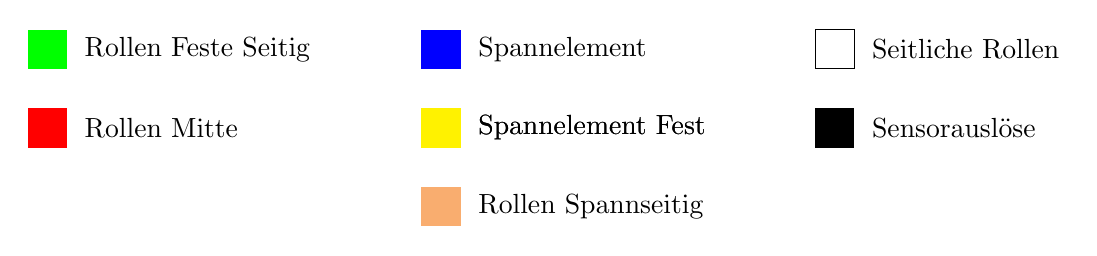
\begin{tikzpicture}
        \fill[green] (0,0) rectangle (0.5,0.5);
        \node[right] at (0.6,0.25) {Rollen Feste Seitig};
        \fill[red] (0,-1) rectangle (0.5,-0.5);
        \node[right] at (0.6,-0.75) {Rollen Mitte};
        \fill[blue] (5,0) rectangle (5.5,0.5);
        \node[right] at (5.6, 0.25) {Spannelement};
        \fill[yellow] (5,-1) rectangle (5.5, -0.5);
        \node[right] at (5.6,-0.75) {Spannelement Fest};
        \draw[black] (10,0) rectangle (10.5, 0.5);
        \node[right] at (10.6, 0.25) {Seitliche Rollen};
        \fill[black] (10,-1) rectangle (10.5,-0.5);
        \node[right] at (10.6,-0.75) {Sensorauslöse};
        \fill[yellow] (5,-1) rectangle (5.5, -0.5);
        \node[right] at (5.6,-0.75) {Spannelement Fest};
        \fill[Apricot] (5,-2) rectangle (5.5, -1.5);
        \node[right] at (5.6,-1.75) {Rollen Spannseitig};

    \end{tikzpicture}
    \caption{X-Achse}
    \label{X-Achse_ansichten}
\end{figure}


\begin{figure}[H]
    \centering
    \begin{subfigure}{.5\textwidth}
        \centering
        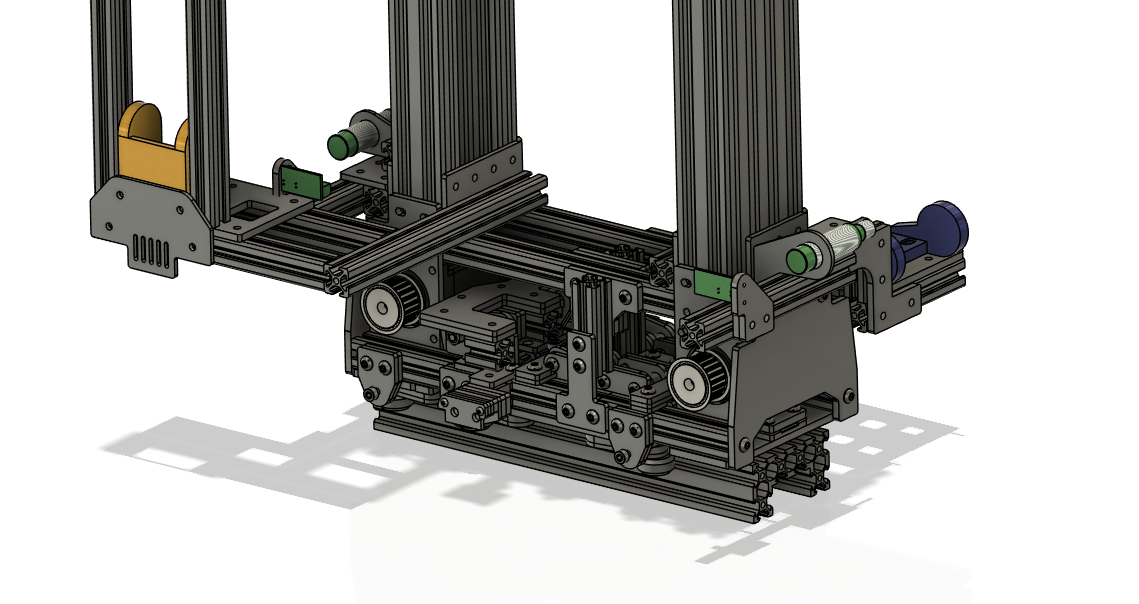
\includegraphics[width=0.94\textwidth]{X-Achse_b1.png}
        \caption{X-Schuttle unten mit Anbauten}
        \label{X-Achse_b1}
    \end{subfigure}%
    \begin{subfigure}{.5\textwidth}
        \centering
        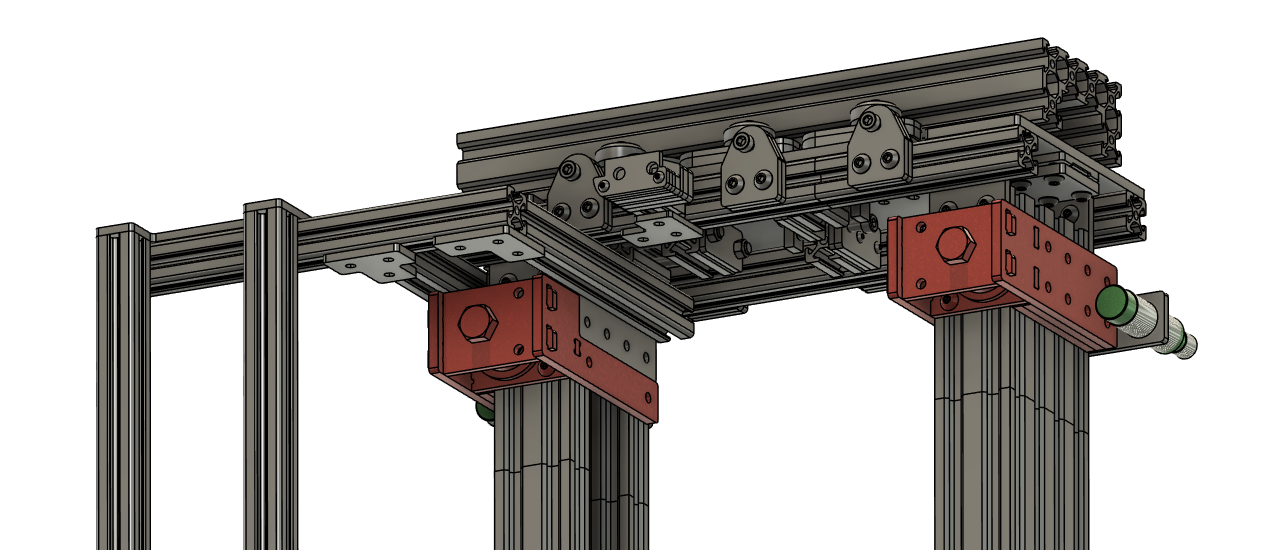
\includegraphics[width=0.94\textwidth]{X-Achse_b2.png}
        \caption{X-Shuttel oben}
        \label{X-Achse_b2}
    \end{subfigure}
    %caption with boxes of color as legend and a descritption for the color, side by side
    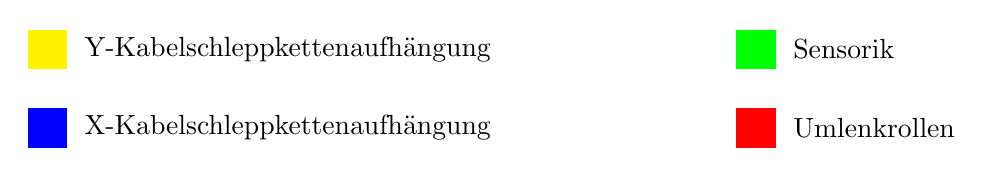
\begin{tikzpicture}
        \fill[yellow] (0,0) rectangle (0.5,0.5);
        \node[right] at (0.6,0.25) {Y-Kabelschleppkettenaufhängung};
        \fill[blue] (0,-1) rectangle (0.5,-0.5);
        \node[right] at (0.6,-0.75) {X-Kabelschleppkettenaufhängung};
        \fill[green] (9,0) rectangle (9.5,0.5);
        \node[right] at (9.6, 0.25) {Sensorik};
        \fill[red] (9,-1) rectangle (9.5, -0.5);
        \node[right] at (9.6,-0.75) {Umlenkrollen};
        
    \end{tikzpicture}
    \caption{X-Achse Gesamtansichten}
    \label{X-Achse_ansichten2}
\end{figure}


\subsubsection{Y-Achse}
Als Y-Achse wird jene Achse bezeichnet, die ihre Bewegung vertikal durchführt. Sie hat die Aufgabe, die Z-Achse bzw. das YZ-Shuttle auf Position zu bringen. Wichtig hierbei ist jedoch, dass die Y-Achse die Aufgabe des Aufhebens der Box übernimmt.

\paragraph{Antriebsauslegung}\mbox{}\\
Dadurch, dass die Y-Achse sowohl das YZ-Shuttle als auch die Boxen aufheben muss, muss der Antrieb dementsprechend dimensioniert werden. Als Formfaktor soll ein Nema23-Schrittmotor verwendet werden. Diese sind weit verbreitet und im Vergleich zu Servomotoren relativ kostengünstig. Als Grundformfaktor wird ein \SI{2}{\newton\meter} Motor gewählt. Nun soll überprüft werden, ob dieser die Last der YZ-Achse auch antreiben kann.

\vspace{5mm}
\noindent\begin{minipage}{\textwidth}
\begin{minipage}[t]{0.5\textwidth}
    \begin{equation*}
        F = \frac{M}{\frac{d}{2} \cdot 1000} \cdot n
    \end{equation*}
    \begin{equation*}
        F = \frac{2 \uni{Nm}}{\frac{30 \uni{mm}}{2} \cdot 1000} \cdot 2 = 266 \uni{N}
    \end{equation*}
\end{minipage}%
\begin{minipage}[t]{0.4\textwidth}
    \vspace*{-5mm}
    \begin{align*}
        &F: \text{Antriebskraft der Y-Achse} & &\left[N\right]\\
        &M: \text{Drehmoment eines Motors} & &\left[Nm\right]\\
        &d: \text{Durchmesser der Zahnscheibe} & &\left[mm\right]\\
        &n: \text{Anzahl der Antriebe} & &
    \end{align*}
\end{minipage}
\end{minipage}
\vspace{5mm}

Bei der Konstruktion einer früheren Version des YZ-Shuttles wurde erfasst, dass das Shuttle bis zu \SI{13}{\kg} wiegen kann. Dies wird zwar in einer späteren Iteration des Designprozesses noch verbessert, dient jedoch als Richtwert für die Antriebsauslegung. \SI{13}{kg} erzeugen ohne Berücksichtigung von Reibung knapp  \SI{130}{\newton}. Die Antriebskraft der Schrittmotoren reicht auf jeden Fall aus. Doch diese Überdimensionierung ist unter dem Aspekt, dass die Antriebe über keine Bremse verfügen und somit das gesamte Gewicht der Z-Achse sowie der Kabelschleppkette immer unterstützt werden müssen, durchaus sinnvoll.

\paragraph{Zahnriemen und Umlenkung}\mbox{}\\
Als Zahnriemen wird auch bei der Y-Achse auf ein AT5x16-Profil gesetzt. Doch hier gestaltet sich die Positionierung ebendieses nicht so simpel wie bei der X-Achse. Da der Zahnriemen beim YZ-Shuttle an einem bestimmten Punkt befestigt werden muss, muss er auch dort wieder rückgeführt werden. Die Umlenkung des Zahnriemens gestaltet sich jedoch wesentlich anspruchsvoller als bei der X-Achse, da einerseits ein möglichst kompakter Formfaktor angestrebt werden muss und andererseits eine aufhängungstechnisch sehr unvorteilhafte Positionierung vor dem V-Slot-C-Profil erforderlich ist. Aus diesem Grund wird eine Konstruktion aus Aluminium, welche sich selbst verhakt, konstruiert (siehe \ref{X-Achse_b2}). Sie muss seitlich an den Profilen verschraubt werden. Im vorderen Überhang werden Aluminiumelemente eingehängt, die die Aufhängung der Achse für die Umlenkung erlauben.

\paragraph{Zahnriemenaufgängung}\mbox{}\\
Um die optimale Position der Zahnriemenaufhängung für die Y-Achse bestimmen zu können, wird überschlagsmäßig ein Massenschwerpunkt in Z-Richtung berechnet. Um mit der Konstruktion beginnen zu können, werden hierfür ungefähre Werte angenommen.

\noindent\begin{minipage}{\textwidth}
\begin{minipage}[t]{0.5\textwidth}
    \vspace{7mm}
    \begin{equation*}
        Z_s = \frac{1}{M} \cdot \displaystyle\sum_{i = 0}^{n} z_i \cdot m_i
    \end{equation*}
\end{minipage}%
\begin{minipage}[t]{0.5\textwidth}
    \begin{align*}
        &Z_s: \text{Position des Massenschwerpunkts} & &\left[m\right]\\
        &M: \text{Gesamtmasse} & &\left[kg\right]\\
        &z_1: \text{Z-Koordinate der Teilmasse} & &\left[m\right] \\
        &m_1: \text{Masse der Teilmasse} & &\left[kg\right]
    \end{align*}
\end{minipage}
\end{minipage}

\begin{table}[H]
    \centering
    \centering
        \begin{tabular}{c c c}
            Gegenstand & Masse in kg & Position in mm\\
            \hline
            Motor & 0.3 & 21 \\
            Z-Schiene & 1 & 150 \\
            Z-Gable & 0.3 & 180 
        \end{tabular}
    \caption{X-Achse unbeladen und eingefahren}
        \vspace{5mm}
        \centering
        \begin{tabular}{c c c}
            Gegenstand & Masse in kg & Position in mm\\ 
            \hline
            Motor & 0.3 & 21 \\
            Z-Schiene & 1 & 150 \\
            Z-Gabel & 1.3 & 380
        \end{tabular}
        \caption{X-Achse beim Ladevorgang}
\end{table}
So werden zwei Schwerpunkte errechnet: ca. \SI{130}{\mm} im unbeladenen Zustand und 250 mm während dem Ladevorgang. Da die Stabilität des Y-Shuttles während dem Ladevorgang wichtiger ist als während einer Leerfahrt, wird das Y-Shuttle so positioniert, dass die Aufhängung des Zahnriemens bei rund 200 mm liegt.\\
Weiters muss auch dieser Zahnriemen wieder gespannt werden. Durch die geringere Zahnriemenlänge wird auch der Spannmechanismus verkleinert.
Leider muss dieser aus Platzgründen außerhalb der Flucht zum Zahnriemen angebracht werden. Die Folgen dieser Auslenkung auf die Riemenspannung können durch folgenden Ausdruck, der die Länge, die der Zahnriemen bei einer bestimmten Position braucht, um spannungslos zu sein, approximiert, ermittelt werden. (Hierbei wird von einem linearen Zusammenhang zwischen der Kraft auf die Aufhängung und der Längenkontraktion ausgegangen. In der Realität würde jedoch die Elastizität des Zahnriemens sowie jene der Aufhängung Auswirkungen haben, aber diese verringern die Auswirkungen).
\\

    \noindent\begin{minipage}{\textwidth}
        \vspace{4mm}
    \begin{minipage}[t]{0.5\textwidth}
        \begin{equation*}
            K(h) = \sqrt{h^2+d^2}+(l-h)
        \end{equation*}
        \begin{equation*}
            K(h) = \sqrt{h^2+28^2}+(1500-h)
        \end{equation*}
    \end{minipage}%
    \begin{minipage}[t]{0.5\textwidth}
        \vspace{-7mm}
        \begin{align*}
            &K(h): \text{theoretische Länge des Riemen} & &\left[mm\right]\\
            &h: \text{Position des Schlittens} & &\left[mm\right]\\
            &l: \text{Umlenkungsrollenabstand} & &\left[mm\right]\\
            &d: \text{Abstand der Klemme zur Flucht} & &\left[mm\right]
        \end{align*}
    \end{minipage}
    \end{minipage}

    \begin{figure}[H]
        \centering
        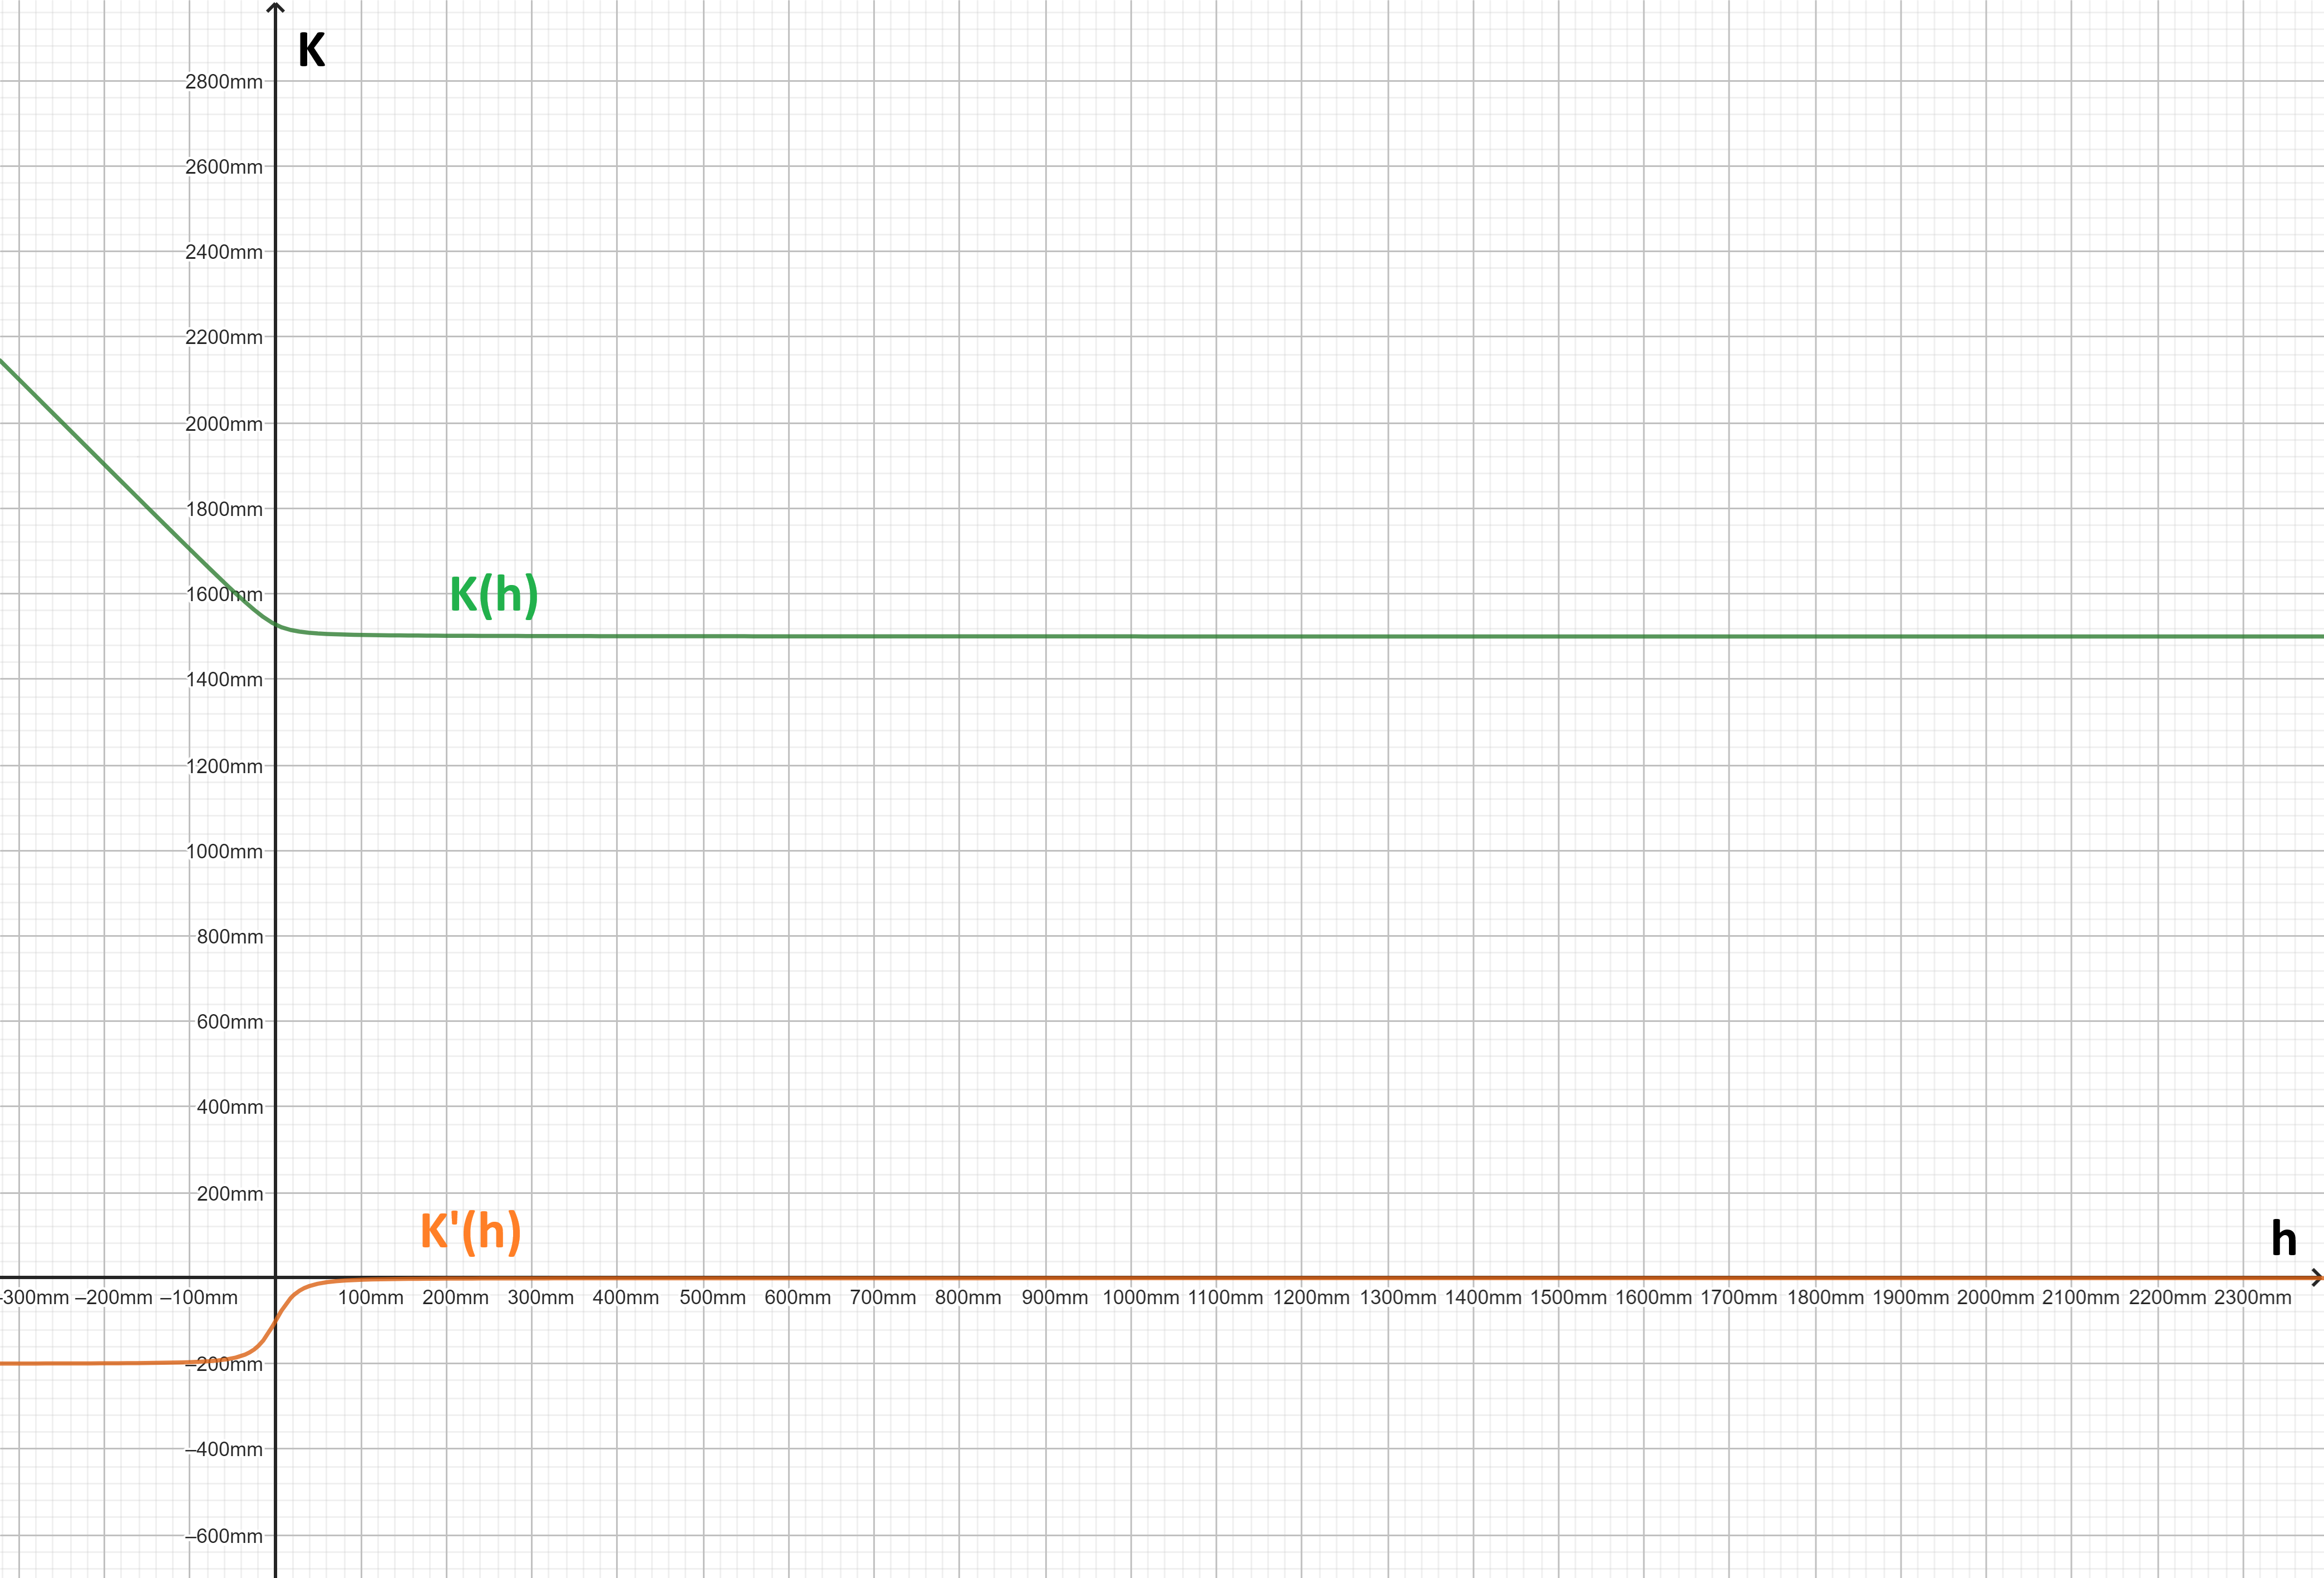
\includegraphics[width=0.7\textwidth]{Zahnrimenenversatz.png}
        \caption{Zahnriemenkontraktion grafisch dargestellt}
        \label{zahnriemenversatz}
    \end{figure}

    Aus der Abbildung \ref{zahnriemenversatz} geht, wie schon intuitiv vermutet, hervor, dass diese Asymmetrie nur dann ein Problem darstellt, wenn der Schlitten weit unten ist. Ein konkretes Maß kann folgendermaßen ermittelt werden: \(K(80) - (750) = 4.24\unit{\milli\meter}\). Der Unterschied in der benötigten Riemenlänge zwischen der Mittelstellung (750 \unit{\milli\meter} ) und der Ruheposition (\SI{80}{\mm} über der Zahnscheibe) beträgt also rund \SI{4}{\mm}. Im Hinblick darauf, dass diese Länge auf zwei Seiten (Hin- und Rücklaufseite) des Zahnriemens aufgeteilt wird (welcher etwas elastisch ist), sowie dass eine leichte Biegung in der Umlenkungsaufhängung auftritt, wird diese Extraspannung toleriert.

\paragraph{Shuttleführung}\mbox{}\\
Das YZ-Shuttle wird aus Stabilitätsgründen ebenfalls mit einem V-Slot C-Profil geführt. Diese sind auf beiden Seiten jeweils oben und unten befestigt. Die Länge wird so gewählt, dass die Verwendung eines \SI{1.5}{\meter} langen Profils perfekt ausreicht. Da das YZ-Shuttle wesentlich weniger Kraft auf die Führung auswirkt, können weniger Führungsräder verwendet werden. Die Hauptführungsräder werden so positioniert, dass sich ein Dreieck ergibt. Dieses dient dazu, dass sowohl beim Aufhebevorgang als auch beim Leerlauf immer eine Klemmung um die Führungsschiene entsteht. Hierbei sind jene V-Wheels, welche beim Aufhebevorgang belastet werden, doppelt ausgeführt. Wie schon bei der X-Achse sind auch hier wieder alle V-Wheel-Abstände mit Schrauben einstellbar. Zusätzlich zur Hauptführung sind auch außen jeweils noch zwei Führungsräder angebracht, um das Shuttle zusätzlich zu stabilisieren.\\
Dabei muss die Halterung auf der Zahnriemenseite dünner Ausgeführt werden, da sonst eine Kollision zwischen Riemen und Halterung zustande kommen würde.

\paragraph{Sensoren}\mbox{}\\
Da die Endschalter der Y-Achse kapazitiv ausgeführt sind, muss auf dem Shuttle ein metallisches Gegenstück angebracht sein. Diese stehen oben und unten über und lösen so vor Kollision aus. Um die Sensoren anzubinden, muss auch ein ASi-Client auf dem X-Shuttle angebracht werden.

\paragraph{Kabelschleppkette}\mbox{}\\
Um Versorgung der Z-Achse herstellen zu können, muss eine Kabelschleppkette vom X- zum Y-Shuttle angebracht werden. Ach diese muss leider Sonderanforderungen erfüllen. Da die Versorgung von unten ausgeht, muss die Kabelschleppkette stehend eingebaut werden. Dies ist grundsätzlich eine äußerst ungünstige Situation, da diese Schleppkette der Beschleunigung des X-Shuttles ausgesetzt ist. Um ein Schwingen möglichst zu verhindern, werden seitlich noch Führungselemente angebracht. Außerdem sind die Anschlusselemente fest um die ersten Kettenglieder extra zu unterstützen. \cite{igus_vertikal}

\subsubsection{Z-Achse}
Als Z-Achse oder Gabel, wird jener Teil des AFSS bezeichnet, der die Boxen in das Lager ein- und ausfährt. Dieser ist in das YZ-Shuttel integriert. Es wird davon ausgegangen, dass um Boxen ein- und auszuheben ca. 210 mm überstand der Gabel benötigt wird. Dies ist also der Mindestverfahrweg der Z-Achse

\paragraph{Linearführung}\mbox{}\\
Geführt wird die Gabel mit zwei Führungsschienen von Igus. Diese bieten optimale Stabilität sowie, in Verbindung mit einem Führungswagen, eine reibungsarme Bewegung. Wichtig ist jedoch, dass der Schwerpunkt der am Führungswagen befestigten Last nicht mehr als die doppelte Wagenlänge über den Wagen hinausgeht. Danach kommt es zu sehr starker Verklemmung, und ein Betrieb ist nur mehr schwer möglich. Da bei einer Auslegeroperation der Schwerpunkt sehr weit übersteht, wird eine TS-01 Führungsschienen- und -wagenkombination verwendet. Diese wirkt zwar recht überdimensioniert, doch da der Führungswagen so lang ist, kann ein reibungsarmer Betrieb gewährleistet werden.

\paragraph{Motor}\mbox{}\\
Als Antrieb für die Z-Achse sollen zwei Nema-17 Schrittmotoren verwendet werden. Hier ist es nicht nötig, eine Closed-Loop-Steuerung zu verwenden, da bei jedem Hub auch referenziert werden kann. Weiterhin kann dadurch Kabelschleppkettenplatz gespart werden.

\paragraph{Spindelauslegung}\mbox{}\\
Die Z-Achse wird mit einer Spindel angetrieben. Dies bietet Vorteile in der Positionsgenauigkeit und der Kraftübertragung. Jedoch ist es wichtig, die richtige Spindelsteigung auszuwählen, um die Balance zwischen Geschwindigkeit und Kraft zu halten. Ziel ist es, für eine Richtung des Hubs maximal 5 Sekunden zu benötigen. Sie wird über eine Zahnscheibe und Zahnriemen mit dem Motor verbunden.\\
Berechnet werden kann diese Zeit mit folgendem Ausdruck:

\vspace{5mm}
\noindent\begin{minipage}{\textwidth}
\begin{minipage}[t]{0.5\textwidth}
    \vspace{10mm}
    \begin{equation*}
        v = \frac{k}{n_{welle}} = \frac{k}{\frac{n_{motor}}{i}}
    \end{equation*}
    \begin{equation*}
        F = \frac{M_{mot} \cdot i \cdot k}{n_{welle}} \cdot 2 \pi f \cdot \eta 
    \end{equation*}
\end{minipage}%
\begin{minipage}[t]{0.5\textwidth}
    \vspace{-7mm}
    \begin{align*}
        &M_{mot}: \text{Drehmoment} & &\left[\frac{N}{m}\right]\\
        &n_{mot}: \text{Drehzahl} & &\left[\frac{1}{s}\right]\\
        &k: \text{Wellensteigung} & &\left[\frac{mm}{U}\right]\\
        &i: \text{Übersetzungsverhältniss} & \\
        &\eta: \text{Wirkungsgrad der Gewindeshraube} & \\
    \end{align*}
\end{minipage}
\end{minipage}

\vspace{5mm}

So wird berechnet, dass eine DS10x12-Spindel mit ihrer \SI{12}{\mm} Steigung, bei einer Motordrehzahl von {\SI{600}{\Umdrehung\per\minute}} (\SI{0.42}{\newton\meter}) und einem Übersetzungsverhältnis von 2:1, ca. 4 Sekunden pro Richtung benötigt und mit einer Kraft von ca. \SI{90}{\newton} bewegt wird.\\
Dies entspricht unseren Anforderungen, und somit wird diese Spindel gewählt. Um sie zu lagern, wird vorne und hinten der Durchmesser der Spindel verringert, sodass diese in Kugellagern geführt werden kann.

\paragraph{Sensorik}\mbox{}\\
Um auch die Endschalter der Z-Achse, sowie weitere Sensoren einzulesen, wird auch hier ein ASi-Slave montiert.


\begin{figure}[H]
    \centering
    \begin{subfigure}{.5\textwidth}
        \centering
        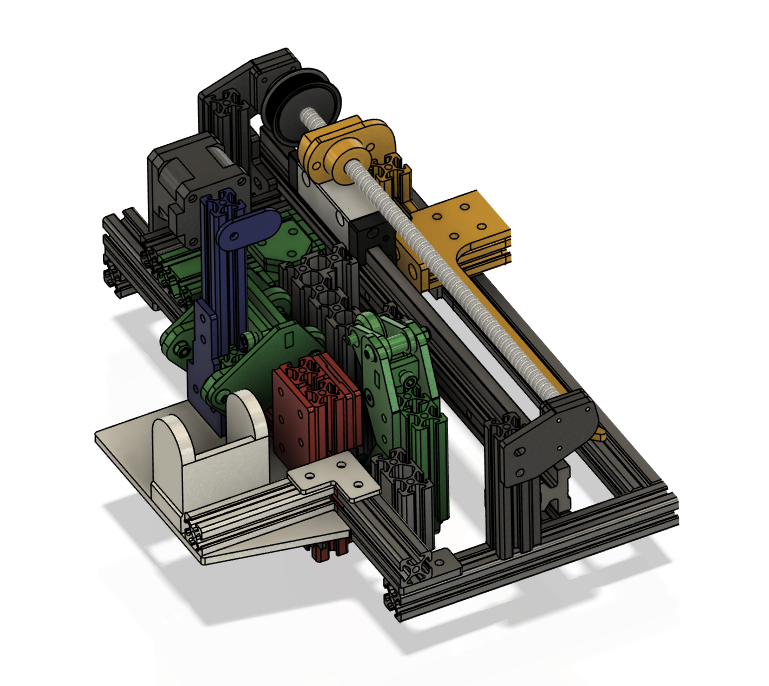
\includegraphics[width=0.94\textwidth]{yz-schnitt1.png}
        \caption{YZ-Achse, zweite Hälfte ausgeblendet}
        \label{yz-schnitt1}
        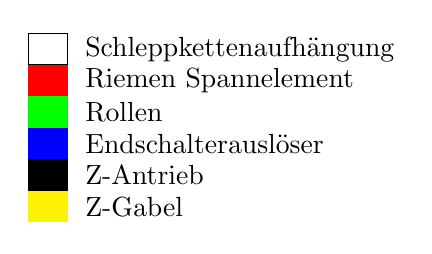
\begin{tikzpicture}
            \draw[black] (0,0.2) rectangle (0.5, -0.2);
            \node[right] at (0.6,0) {Schleppkettenaufhängung};

            \fill[red] (0,-0.2) rectangle (0.5, -0.6);
            \node[right] at (0.6,-0.4) {Riemen Spannelement};

            \fill[green] (0,-0.6) rectangle (0.5,-1.2);
            \node[right] at (0.6,-0.8) {Rollen};

            \fill[blue] (0,-1) rectangle (0.5,-1.4);
            \node[right] at (0.6,-1.2) {Endschalterauslöser};

            \fill[black] (0,-1.4) rectangle (0.5,-1.8);
            \node[right] at (0.6,-1.6) {Z-Antrieb};

            \fill[yellow] (0,-1.8) rectangle (0.5,-2.2);
            \node[right] at (0.6,-2) {Z-Gabel};
            

        \end{tikzpicture}
    \end{subfigure}%
    \begin{subfigure}{.5\textwidth}
        \centering
        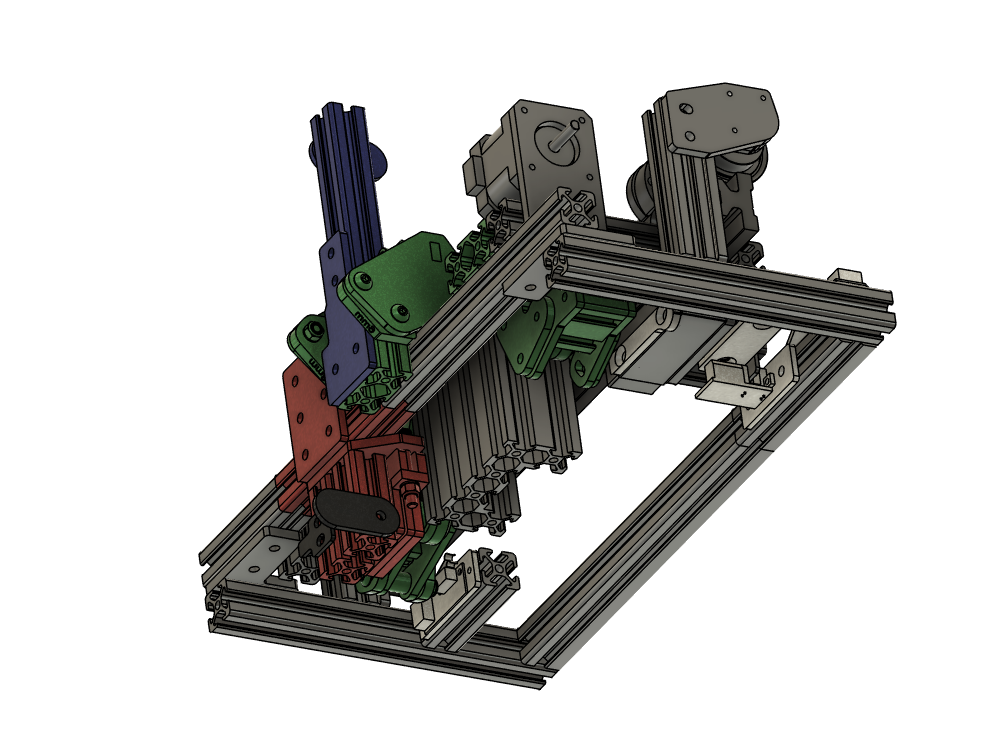
\includegraphics[width=0.94\textwidth]{yz-schnitt2.png}
        \caption{YZ-Achse von unten, zweite Hälfte}
        \label{yz-schnitt2}
        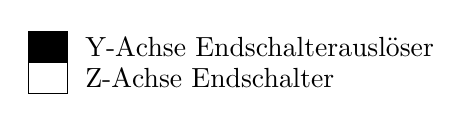
\begin{tikzpicture}
            \fill[black] (0,0.2) rectangle (0.5, -0.2);
            \node[right] at (0.6,0) {Y-Achse Endschalterauslöser};

            \draw[black] (0,-0.2) rectangle (0.5, -0.6);
            \node[right] at (0.6,-0.4) {Z-Achse Endschalter};


        \end{tikzpicture}
    \end{subfigure}
    %caption with boxes of color as legend and a descritption for the color, side by side
    \caption{YZ-Achse}
    \label{YZ-Achse_ansichten}
\end{figure}

\begin{figure}[h]
    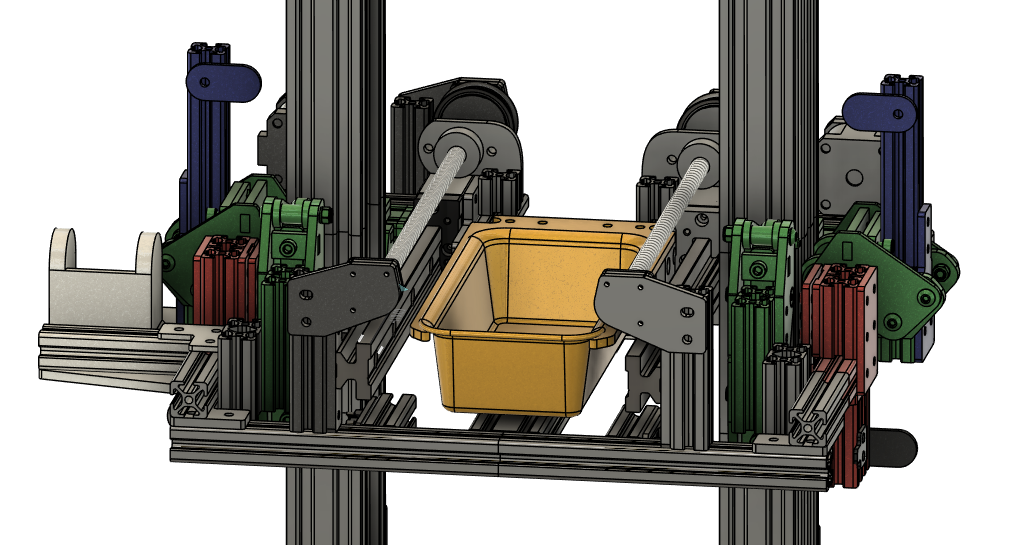
\includegraphics[width=1\textwidth]{yz-full.png}
    \caption{XY-Shuttel Gesamtansicht}
\end{figure}

\subsubsection{Lager}
Das Lager soll die Boxen beinhalten und die Möglichkeit zulassen, dass diese von der Gabel ein- und ausgehoben werden. Weiterhin muss die Box in X- und Z-Richtung geführt werden, um die Positionsgenauigkeit sicherzustellen, da sonst die Gabel möglicherweise in die Box fährt. Das Lager soll darauf ausgelegt werden, dass Boxen mit den Maßen \qtyproduct{50 x 100 x 200}{\milli\metre} verwendet werden können. Diese Boxen sind nach unten hin verjüngt und haben oben eine Lippe, an der die Gabel greift.
Umgesetzt wird dies mit einem Gerüst aus 40x40-Item-Profilen, welches im Nachhinein in den restlichen Rahmen eingesetzt wird. Auf diese werden 20x40-Profile horizontal aufgeschraubt, auf denen die Boxen stehen. Vorne und hinten wird eine Kunststoffplatte aufgeschraubt, welche leicht übersteht und somit die Box in Z-Richtung positioniert. Zwischen den Boxen wird ein Trennsteg eingebaut, welcher die Boxen in X-Richtung positioniert sowie den richtigen Abstand zwischen den Boxen einhält.

\subsubsection{Querförderer}
Da es dem Portalroboter nicht möglich ist, die Boxen direkt auf das Förderband zu legen, muss hier noch ein System eingebaut werden, welches dies erledigt. Da die Boxen beim Ein- und Auslagern den gleichen Weg zurücklegen, muss dieser Querförderer die Box sowohl auf das Förderband als auch vom Förderband herunterbewegen können.\\
Zu diesem Zweck wird eine weitere, der Gabel ähnliche Konstruktion montiert, welche auf einem 20x40-V-Slot-Profil verläuft. Die Box wird dann hin- und hergeschoben, um vom Lager auf das Förderband umzuladen. Dadurch ist es noch möglich, dass die Gabel der Z-Achse die Box in der Nullstellung ein- und aushebt.


\subsubsection{Fertigung der Einzelteile}\nobreak
Die Fertigung der Bauteile erfolgt parallel zur Montage. Hierzu werden viele Tiele Gefräßt, Gelasert und Aluminiumprofile zugeschnitten. Manche Teile sind jedoch komplexer und müssen speziell angefertigt werden.

\paragraph{Umlenkrollen}\mbox{}\\
Die Umlenkrollen sind jeweils am Ende der X- und Y-Achsen angebracht. Da diese der gesamten Spannkraft ausgesetzt sind, erfordert dies spezielle Anforderungen an die Aufhängung sowie an die Umlenkrolle selbst. Diese soll primär eine 180°-Wende des Zahnriemens ermöglichen und sekundär eine Führung für den Riemen bieten.\\
Um diese Anforderungen umzusetzen, werden vier Aluminium-Drehteile gefertigt, in welche Kugellager eingepresst werden.

\begin{figure}[H]
    \centering
    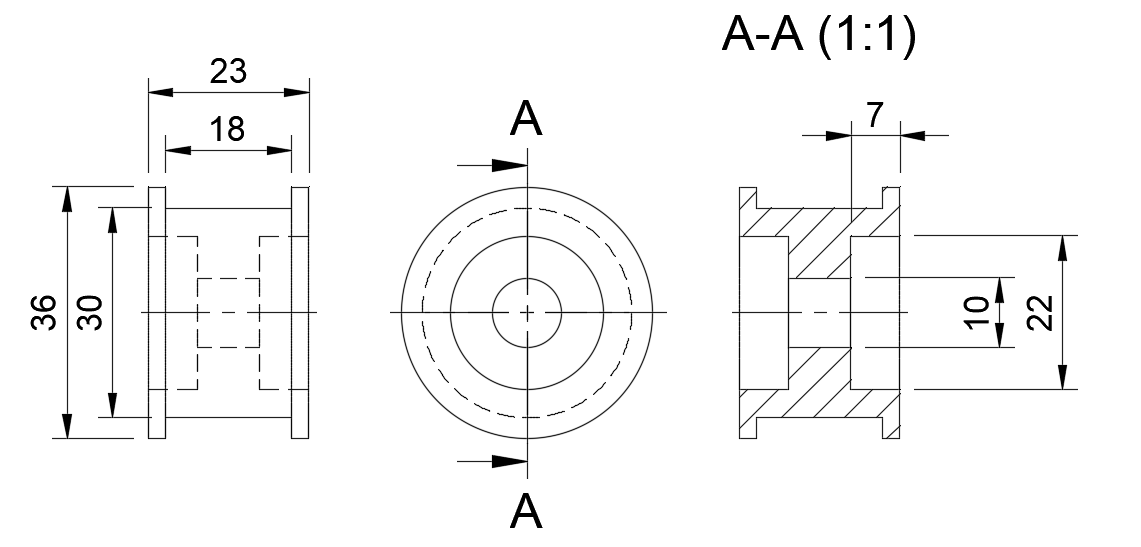
\includegraphics[width=0.8\textwidth]{AT5x16-Umlenkung.png}
    \caption{Bauteilzeichnung Umlenkrolle}
    \label{UmlenkrolleBTZ}
\end{figure}

Die Fertigung dieses Teils nach Abb. \ref{UmlenkrolleBTZ} lässt sich in folgende Teilschritte unterteilen:
\begin{itemize}
    \setlength\itemsep{-1mm} 
    \item Zuerst die Frontfläche plandrehen (Drehzahl: \SI{900}{\Umdrehung\per\minute})
    \item Ungefähr \SI{30}{mm} Länge auf das Aussenmaß von \SI{36}{mm} längsdrehen
    \item Mit \SI{9.8}{mm} Bohrer das mittlere Loch vorbohren (\SI{540}{\Umdrehung\per\minute})
    \item Mit \SI{10}{mm} Reibeisen und viel Öl das Loch auf eine genaue Passung bringen (\SI{260}{\Umdrehung\per\minute})
    \item Die Position relativ zum Backenfutter markieren, um beim Neu-Einspannen Rundlaufgenauigkeit zu gewährleisten
    \item Zylinder bei ca. \SI{26}{mm} abstechen (\SI{540}{\Umdrehung\per\minute})
    \item Umspannen und auf Maß plandrehen (\SI{900}{\Umdrehung\per\minute})
    \item Die Aussparung für die Lager mit Eckdrehmeißel beginnen, jedoch nach innen hin nur \SI{6.8}{mm}
    \item Bei ca. \SI{17}{mm} Lochdurchmesser den tatsächlichen Durchmesser mit der Digitalanzeige vergleichen und gegebenenfalls korrigieren
    \item Bei \SI{21.5}{mm} den Oberschlitten die restlichen \SI{0.2}{mm} zustellen und die gesamte Tiefe plandrehen
    \item Den Lochdurchmesser auf \SI{21.95}{mm} erweitern und dann in kleinen Inkrementen zustellen, bis das Lager gerade so nicht passt, um einen Presssitz zu gewährleisten. Dies tritt bei Lagern mit \SI{22}{mm} Außendurchmesser bei rund \SI{22.045}{mm} ein.
    \item Da für die Einsparung der Riemenführungsfläche kein Angriffspunkt verfügbar ist, wurde als Halterung ein Dorn nach Abb. \ref{ulr:dorn} gedreht, auf welchen das Drehteil aufgeschraubt wird.
    \item Mit dem Abstechmeißel wird in \SI{2}{mm} Inkrementen die Zahnriemenauflagefläche herausgedreht, bis auf \SI{21.95}{mm}, sowie links und rechts den Rand \SI{1}{mm} extra dick lassen (siehe Abb. \ref{ulr:f1} ). (\SI{540}{\Umdrehung\per\minute})
    \item Am Schluss wird die Rand Tiefe auf Maß gedreht.
    \item Als letzten Schritt werden links und rechts die zwei Lager eingepresst.
\end{itemize}

    Durch die verhältnismäßig großen Toleranzen bei den Lageraussendurchmessern wird bei 2 der 8 Lagerpassungen zusätzlich Lagerkleber verwendet, um einen zuverlässigen Halt zu gewährleisten, da bei diesen die Toleranzen nicht eingehalten wurden.\\
    Nach diesem Vorgang sind die vier Umlenkrollen fertig (siehe \ref{ulr:f2}) und können auf einem 8-mm-Schaft montiert werden.

    \begin{figure}[H]
        \centering
        \begin{subfigure}{.3\textwidth}
            \centering
            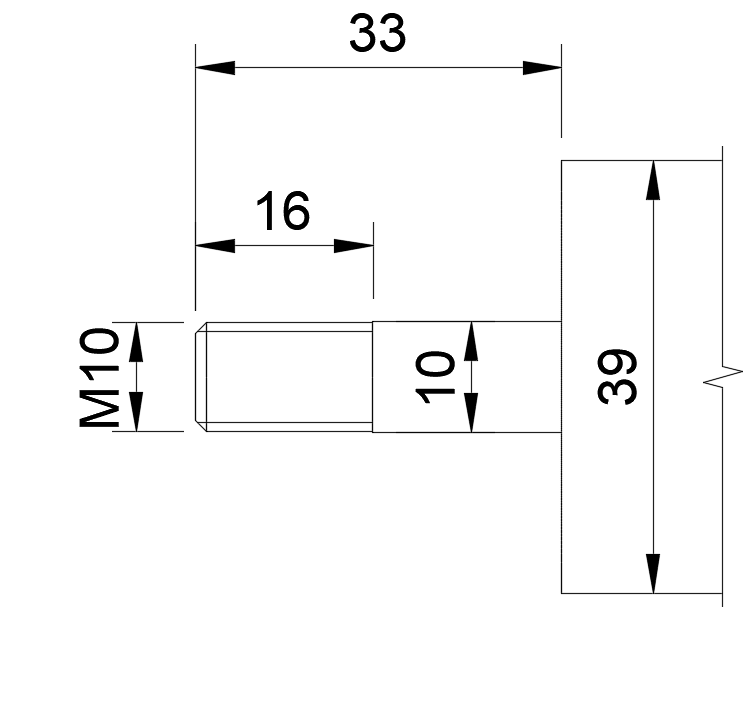
\includegraphics[width=0.9\textwidth]{AT5x16-Umlenkung-Dorn.png}
            \caption{Dorn}
            \label{ulr:dorn}
        \end{subfigure}%
        \begin{subfigure}{.3\textwidth}
            \centering
            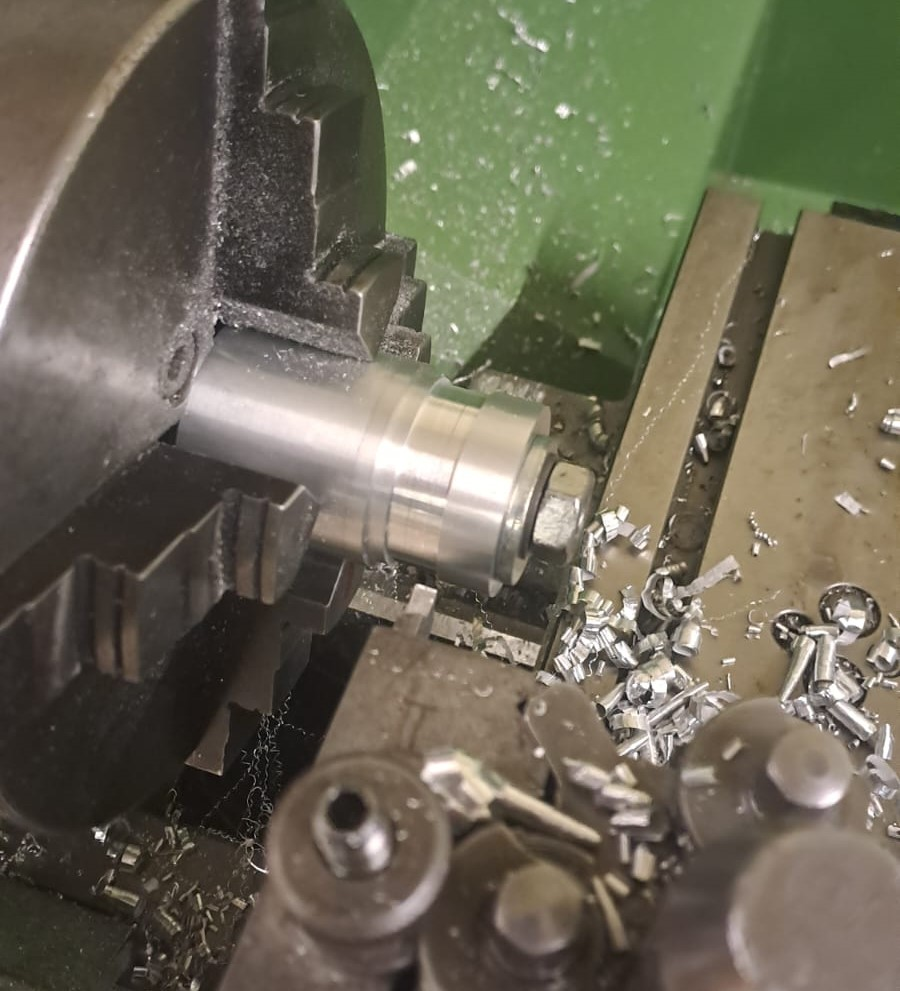
\includegraphics[width=0.9\textwidth]{ulr-fertigung.jpg}
            \caption{Fertigung der Lauffläche}
            \label{ulr:f1}
        \end{subfigure}%
        \begin{subfigure}{.3\textwidth}
            \centering
            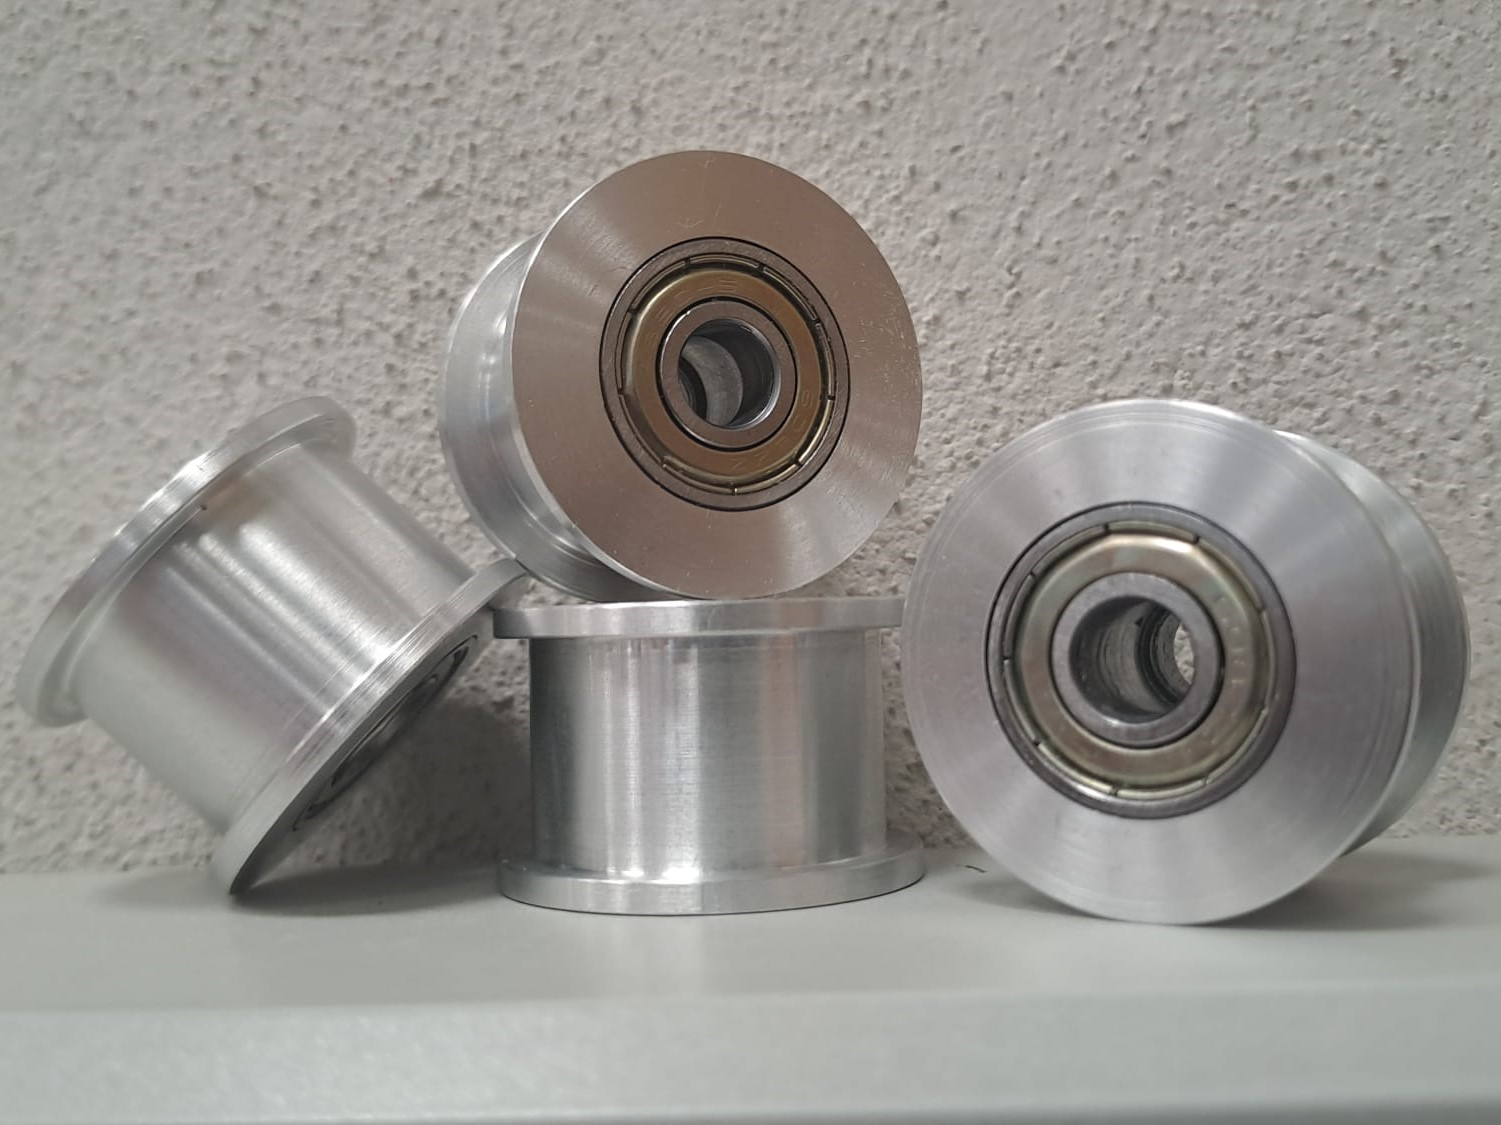
\includegraphics[width=0.9\textwidth]{Umlenkrollen_fertig.jpg}
            \centering
            \caption{Fertiggestellte \\Umlenkrollen}
            \label{ulr:f2}
        \end{subfigure}
        \caption{Umsetzung der Umlenkrollen}
        \label{ulr}
    \end{figure}

\paragraph{Distanzhülsen}\mbox{}\\
Bei den meisten V-Wheels werden Distanzhülsen zur Klemmung benötigt. Diese müssen ein sehr spezielles Maß (\SI{13.4}{\mm} Länge) haben. Deshalb müssen Hülsen mit einer Länge von \SI{20}{\mm} auf diese Länge heruntergedreht werden. Dies wird mit dem rechten Eckdrehmeißel bei einer Drehzahl von \SI{740}{\Umdrehung\per\minute} ausgeführt. Da relativ viele solcher Teile benötigt werden, wird beim Einspannen der Drehmeißel selbst als Endstopp verwendet, um ein relativ wiederholgenaues Maß zu erhalten sowie eine simple Durchführung zu erlauben. Es wird also der Meißel auf Position gefahren und das Werkstück eingespannt, sodass es am Drehmeißel ansteht. Nun wird der Drehmeißel zurückgefahren und die Hülse kann einfach durch mehrere Plandrehoperationen, bis der Schlitten ansteht, gekürzt werden. Es muss also weder gemessen noch die Digitalanzeige verändert werden, um schnell mehrere Teile hintereinander zu fertigen.

\paragraph{Zahnscheiben}\mbox{}\\
Da die Welle des Motors recht kurz ist und die Motoraufhängung Platz wegnimmt, ist es erforderlich, die Zahnscheibe unkonventionell mit dem Motor zu verbinden. Es werden also in der Zahnriemen-Kontaktfläche zwei Löcher gebohrt, angesenkt und mit M4-Gewinde versehen, um dort 2 M4-Wurmschrauben einzuschrauben. Bei der Länge der Wurmschrauben muss darauf geachtet werden, dass sie im montierten Zustand vollständig unter der Oberfläche liegen, um den Zahnriemen nicht zu beschädigen.

\begin{minipage}{\textwidth}
\subsubsection{Aufbau}

Nach Fertigung der Einzelteile kann das AFSS sukksesive zusammengebaut werden.

\paragraph{Rahmen} \mbox{}\\
Gestartet wird mit der Montage des Rahmen. Hierfür werden zuerst alle Aluminiumprofile auf Länge zugeschnitten und Gewinde in den Enden geschnitten. Da nicht genug Profile in der Gesamtlänge des AFSS verfügbar sind, müssen teils noch Verbinder eingesetzt werden. An den Ecken werden die Profile dann mit Standardverbindungssätzen verbunden. Unten werden dann noch die Rollen montiert.

\paragraph{X-Achse} \mbox{}\\
Nachdem die Aufhängungen für die V-Slot Profile gefräßt sind, werden diese an den Rahmen angeschraubt. Auf die V-Slot Profile werden das Nivellierungssystem aufgeschraubt, dann werden die Profile, wie in Abb. \ref{ramreal}, an der Aufhängung befestigt. \\
Danach werden die Umlenkrollen- und die Motoraufhängungen montiert. In diese werden dann Umlenkrollen und Motoren montiert. \\
Nach Fertigung der Bauteile erfolgt auch der zusammenbau des sehr komplexen unteren X-Shuttels relativ reibungslos. Die Stoßverbindung der V-Slot-Profile kann jedoch nicht 100\%ig ausgerichtet werden, deshalb werden dies Übergänge noch abgeschliffen.


\begin{figure}[H]
    \centering
    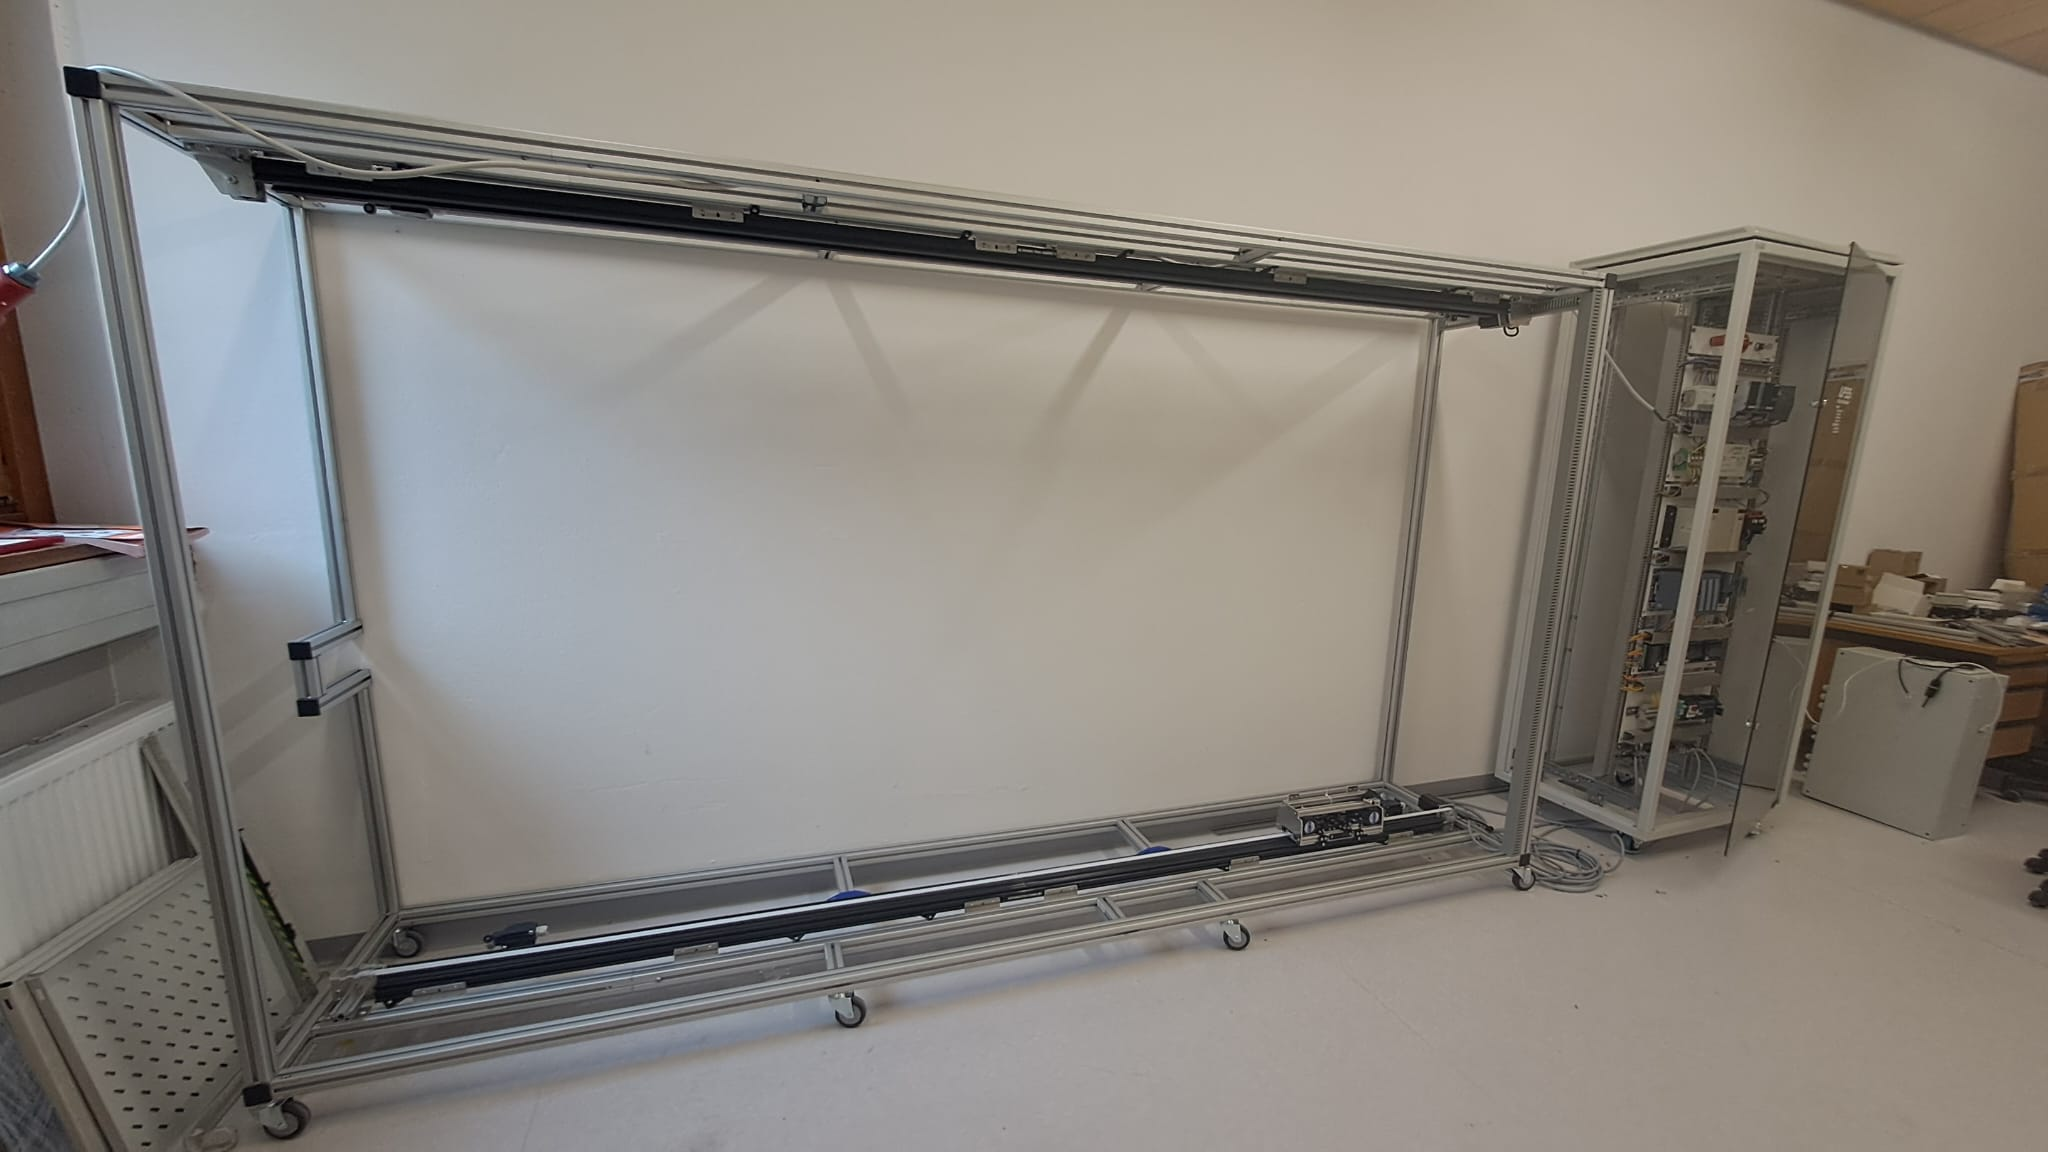
\includegraphics[width=0.9\textwidth]{Rahmen_rael.jpg}
    \caption{Aufgebauter Rahmen und X-Achse}
    \label{ramreal}
\end{figure}

\end{minipage}

\begin{minipage}{\textwidth}
    
\subsubsection{Fazit}
In der Mechanik des AFSS sind nach aktuellem stand über 1000 Bauteile verbaut. Die Umsetzung diese Projekts war nur durch eine sehr umfangreiche theoretische Planung möglich. Zwischen Haupt- und Einzelversionsiterationen wurden mehrere hundert Versionen der Mechanik in Fusion360 durchgeführt. Das dabei erlernte wissen, sowie das daraus resultierende Design, welches viele Aspekte von Fertigung, Wartung und Zusammenbau bedenkt, macht es erst möglich ein solches Vorhaben zu versuchen. Das Gesamtkonstrukt (wie in \ref{AFSS-mech-ges} ersichtlich) beinhält dann die gesamte Mechanik. Erst dadurch, dass eine volle Konstruktion erstellt wurde, war es dann möglich mit den Aufbau zu beginnen. Diese funktionierte, nachdem die Benötigten Teile soweit verfügbar waren, auch Reibungslos.

\begin{figure}[H]
    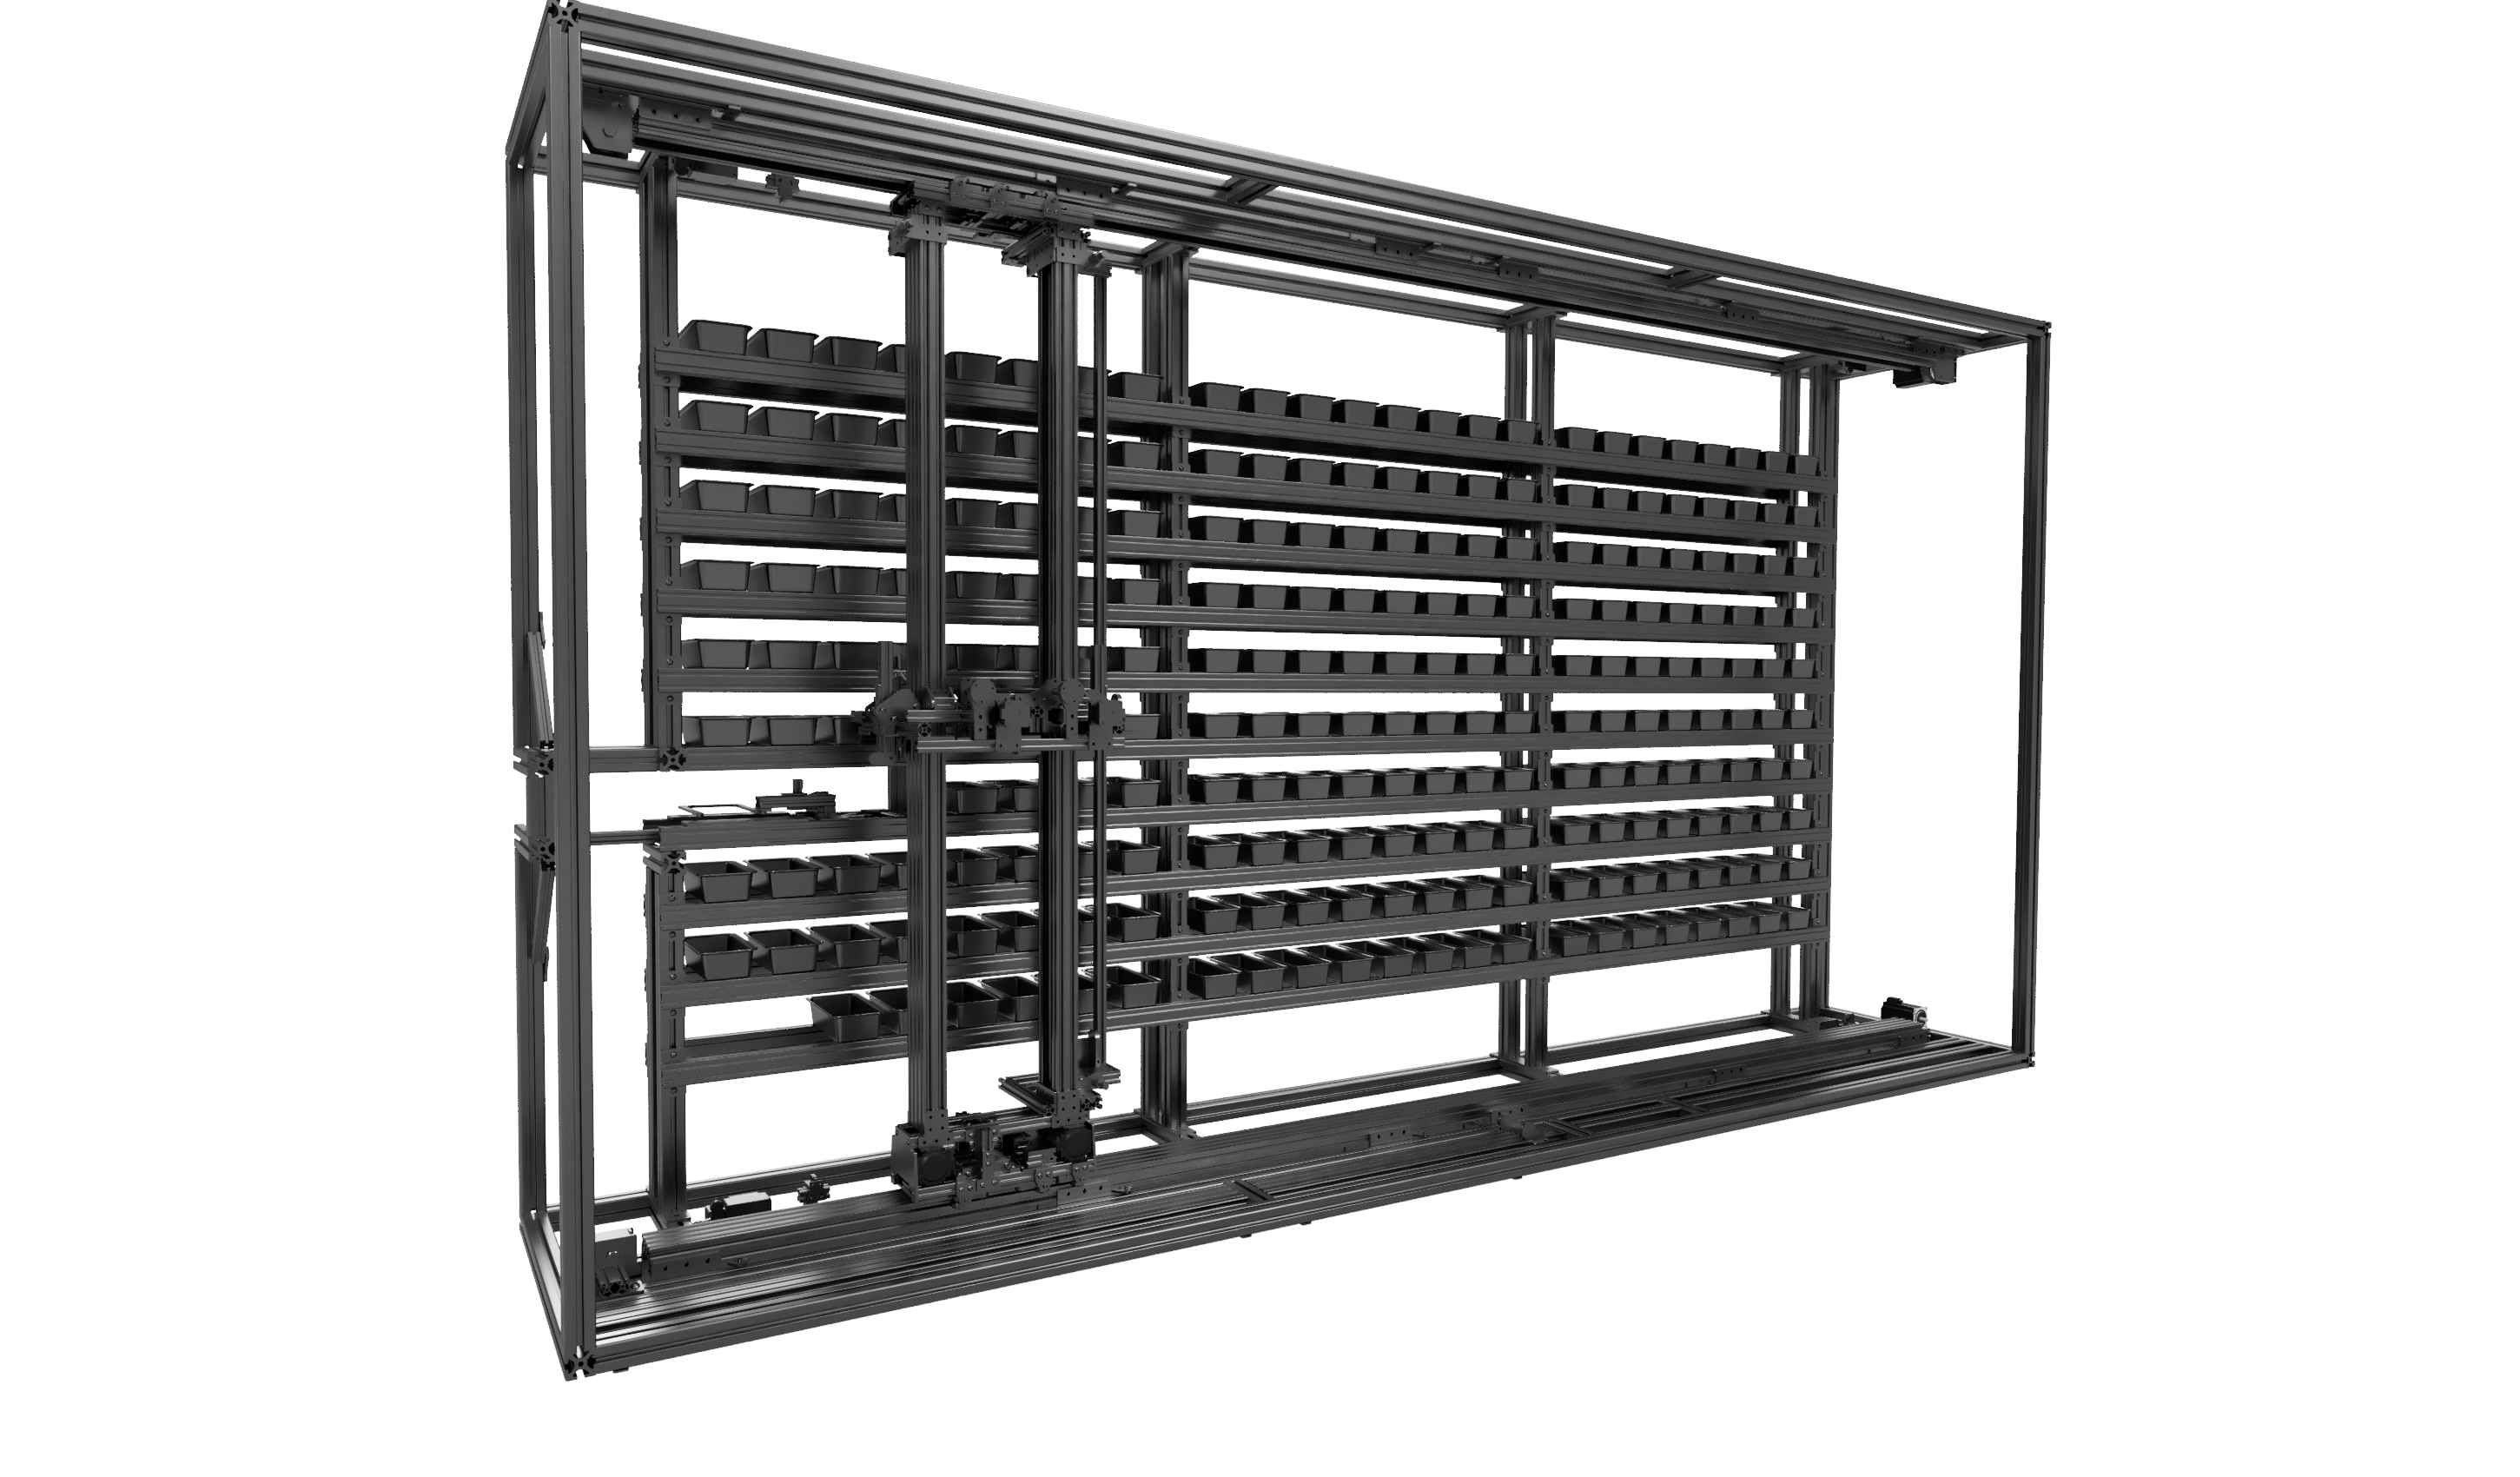
\includegraphics[width=0.9\textwidth]{mech_gesamt.PNG}
    \caption{Gesamtkonstruktion}
    \label{AFSS-mech-ges}
\end{figure}
    
\end{minipage}


\newpage
\subsection{Software und Benutzeroberfläche}

\subsubsection{Grundlegendes}
Um dem Endnutzer die Möglichkeit zu geben, das AFSS möglichst einfach zu bedienen und die komplexe Logik der Lagersteuerung auszuführen, bedarf es eines Servers (Backend) und einer grafischen Benutzeroberfläche (GUI oder Frontend). Diese müssen eine Vielzahl an verschiedenen Funktionen beinhalten.

\subsubsection{Aufbau}
\begin{figure}[h]
    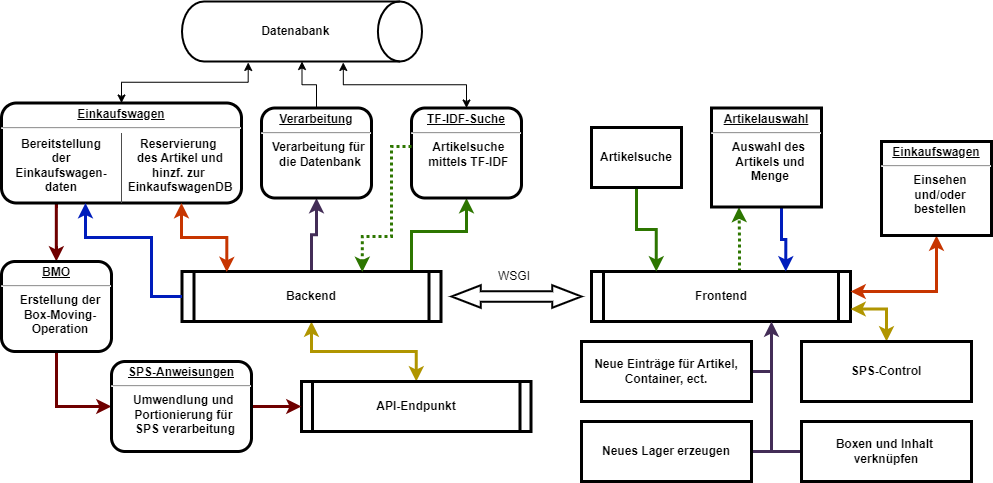
\includegraphics[width=\textwidth]{Software Howl.drawio.png}
    \caption{Gesamtüberblick des Servers}
\end{figure}

Um diesen Anforderungen gerecht zu werden, muss eine Lösung mit sehr hohem Grad an Freiheit in der Logik sowie der UI-Gestaltung gewählt werden. Weiters muss es möglich sein, dass zukünftige Schülerinnen und Schüler diese instand halten und erweitern. Aus diesen Gründen, sowie den bereits vorhandenen Kenntnissen, wird die Programmiersprache 'Python' als Grundlage des Servers verwendet.

\paragraph{Python}\mbox{}\\
Python ist eine vielseitige und hochentwickelte Programmiersprache, die für ihre Einfachheit und Lesbarkeit bekannt ist und sich sowohl für Anfänger als auch für Fortgeschrittene eignet. Sie unterstützt mehrere Programmierphilosophien, darunter objektorientierte und funktionale Programmierung, und wird in Bereichen wie Webentwicklung, Datenanalyse, künstliche Intelligenz und wissenschaftlichem Rechnen häufig eingesetzt. (vgl. \cite{gpt_python})

\paragraph{Flask}\mbox{}\\
Flask ist ein leichtgewichtiges Web-Framework für Python, das durch seine Einfachheit und Flexibilität hervorsticht und sich ideal für kleinere Anwendungen oder Prototypen eignet. Es folgt einem minimalistischen Ansatz, bietet aber Erweiterungsmöglichkeiten, um komplexere Projekte zu realisieren. (vgl. \cite{gpt_flask})

\paragraph{Python - Virtuelle Umgebung}\mbox{}\\
Dieses Projekt enthält sehr viele externe Bibliotheken. In Python sind diese Bibliotheken mit dem Interpreter verknüpft, da bei der Installation diese externen Bibliotheken direkt beim Interpreter gespeichert werden. So kommt es jedoch dazu, dass, wenn das Programm auf einer anderen Maschine ausgeführt wird, diese Bibliotheken nicht vorhanden sind. Um Abhängigkeitskonflikte und Portabilitätsprobleme zu verringern, werden virtuelle Umgebungen verwendet. Diese enthalten den Interpreter sowie die Bibliotheken und könnten einfach auf eine andere Maschine kopiert werden.\\ Dies ist jedoch bei diesem Projekt nur bei der Entwicklung vonnöten, da es bei Fertigstellung im Docker-Container ausgeführt wird.

\subsubsection{Benutzeroberfläche}

Um die Benutzeroberfläche zu realisieren, muss eine Weboberfläche erstellt werden. Auf dieser werden alle Inhalte angezeigt, die für die Benutzung nötig sind. Sie wird vom Server zur Verfügung gestellt, sobald dieser eine HTTP-Anfrage erhält. Um diese mit eigenen Inhalten und Funktionen zu befüllen, muss dies mit HTML geschehen.

\paragraph{HTML}\mbox{}\\
HTML (HyperText Markup Language) ist die Standard-Auszeichnungssprache zur Strukturierung und Darstellung von Inhalten im Web. Sie definiert die grundlegende Struktur einer Webseite mit Elementen wie Überschriften, Absätzen, Links, Bildern und Formularen. (vgl. \cite{gpt_html})\\

Dadurch, dass sich viele Elemente des UI wiederholen, wie z. B. die Navigationsleiste, bietet Flask die Möglichkeit, sogenannte 'Templates' zu verwenden. Diese können einmal definiert und dann an mehreren Teilen der Webseite verwendet werden.
Um Elemente wie Formularfelder oder Datenanzeige einfach mit den benötigten Daten anzuzeigen, gibt es die Möglichkeit, Makros zu erstellen, die von Flask mit den bestimmten Daten vorgerendert und in das restliche HTML eingefügt werden.
Um HTML, welches grundsätzlich ohne Formatierung auskommt, zu stylen, muss CSS verwendet werden.

\paragraph{CSS}\mbox{}\\
CSS (Cascading Style Sheets) ist eine Stylesheet-Sprache, die verwendet wird, um das Design und Layout von Webseiten zu gestalten. Sie ermöglicht die Trennung von Inhalt und Darstellung, indem sie Farben, Schriftarten, Abstände und andere visuelle Aspekte definiert. (vgl. \cite{gpt_css})\\

Da auch Logik in der Webseite verbaut werden muss, muss zusätzlich auch Javascript verwendet werden, da HTML und CSS alleine, noch nicht gut genug mit dem Server Kommunizieren können.

\paragraph{JavaScript}\mbox{}\\
JavaScript (JS) ist eine vielseitige Programmiersprache, die hauptsächlich verwendet wird, um interaktive und dynamische Elemente auf Webseiten zu erstellen. Sie läuft direkt im Browser und ermöglicht Funktionen wie Animationen, Formularvalidierungen und die Kommunikation mit Servern in Echtzeit. (vgl. \cite{gpt_js})\\

Praktisch geschieht diese Server-Kommunkation immer mithilfe diese Programmblocks:

\begin{lstlisting}[language=JavaScript, caption=XHR-Kommunikationsblock]
    function sendData(data, callback) {
        var xhr = new XMLHttpRequest();
        var url = "{{url_for('main.add_stock')}}"; //Flask markup, um die richtige url zu erreichen, dies wird vor ausgabe auf der Webseite noch eingesetzt

        xhr.open("POST", url, true);
        xhr.setRequestHeader("Content-Type", "application/json");

        xhr.onreadystatechange = function () {
            if (xhr.readyState === 4 && xhr.status === 200) {
                callback(xhr.responseText)  //die funktion wir aufgerufen
            }
        };
        var jsonData = JSON.stringify(data);
        xhr.send(jsonData);
    }
\end{lstlisting}

Dieser ermöglicht die Übergabe von Daten im JSON format, und einer Funktion, die die zurückgeschickten Daten verarbeitet. In der Praxis wird dieser so aufgerufen:

\begin{lstlisting}[language=JavaScript, caption=JSON-Beispiel]
function add_to_db(){
    sendData({"add_stock": {"barcode": barcode, "quantity": quant, "article": article}}, 
    set_gen_stock)
}

function set_gen_stock(req){
    document.getElementById("generated").innerHTML = req
}\end{lstlisting}

Wie im Quellcode ersichtlich, werden Daten aus der Webseite ausgelesen und in JSON konvertiert. Danach werden diese Daten zusammen mit einer Funktion an 'send\_Data' übergeben. Wie bereits erwähnt, gibt der Server dann Daten zurück. In diesem Fall werden dann Daten aus der DB vorformatiert. Diese werden dann in der zuvor übergebenen Funktion in die Webseite eingefügt.

\subsubsection{Backend}
Das Backend des Servers ist für die Datenverarbeitung verantwortlich. Es ist, wie bereits erwähnt, in Python geschrieben und stellt mit dem Flask-Framework die Benutzeroberfläche zur Verfügung. \\
Aufgebaut ist es in mehrere Bereiche: Einerseits die Webanwendung sowie die API (Application Programming Interface, Schnittstelle zwischen Anwendungen), die Anbindung an die Datenbank, die Verarbeitung der SPS-Befehle und auch der Zugriff auf die SPS.



\paragraph{Serverseite der Benutzeroberfläche}\mbox{}\\
In Flask könne 'bleuprints' definiert werden. Dies sind Webseitelemente die einen Bestimmten URL-Vorsatz haben. So werden anfanges 'blueprints' für Hauptfunktionen ('/', also ohne Vorsatz), Datenbankinteraktionen ('/db\_interactions') usw. definiert. Die Funktionen dafür werden dann in jeweils eigenen Dateien geschrieben. Dies ermöglicht eine weit aus bessere Übersicht bei großen Projekten. \\
Eine Funktion, die für die Verarbeitung der Anfragen einer bestimmten URL verantwortlich ist, sieht immer ähnlich aus.

\begin{lstlisting}[language=Python, caption=Blueprint Beispiel]
    @main.route("/add_stock", methods=["GET", "POST"])
    def add_stock():
        if request.method == "POST":
            if request.data:
                req = request.get_json()

                if "add_stock" in req.keys():
                    dt = req["add_stock"]
                    new = Stock(
                        container=db.session.query(Container)
                        .filter_by(barcode=dt["barcode"])
                        .first()
                        .id,
                        article=dt["article"],
                        quantity=dt["quantity"],
                    )
                    db.session.add(new)
                    db.session.commit()
                    return "Sucsess"

        return render_template("add_stock.html")
\end{lstlisting}  


Anfangs wird mit einem Decorator (@main.route(...)) die gewünschte URL, sowie unterstützte http-Requests definiert. Decoratoren verändern oder erweitern die Eigenschaften von Funktionen. In diesem Fall wird in der Funktion (def ...()) definiert was geschieht, wenn ein erlaubter Request an der URL 'add\_stock' eintrifft. Dieser Funktionsname kann auch in den Flask-Vorlagen verwendet werden um URLs dynamisch zu vergeben.\\
Weiters wird sortiert um welche art von Art von Anfrage es sich handelt. Bei GET-Anfragen wird typischerweise einfach nur das HTML der Webseite zurückgegeben. Bei POST-Anfragen werden zuerst die Daten dieser Anfrage eytrahiert und dann entschieden was damit gemacht werden soll. In diesem Fall wird, wenn des richtige Schlüsselwort in der Anfrage enthalten ist, ein Datenbankeintrag, mit den Daten aus dem Request, hinzugefügt. Schlussendlich wird ein Wert zurückgegeben, entweder ein HTML-Statuscode, vorgerendertes HTML oder, wie in diesem Fall, ein Text.

\subsubsection{APIs}

\paragraph{SPS - Verbindung}\mbox{}\\
Die Daten für die SPS werden in einem Ähnlichen vefahren zu verfügung gestellt. Nun schickt nicht die Benutzeroberfläche oder der Browser eine Anfrage an das Backend, sondern die SPS. Der Programmblock zur Verarbeitung dieser Anfrage sieht folgenderaßen aus:

\begin{lstlisting}[language=Python, caption={Schnittstelle für die SPS}]
@api.route("/afss", methods=["GET", "POST"])
def afss():   
    request_data = {...} #aus platzgruenden verkuerzt
    if request.method == "POST":
        ... # Abfrage ob der Sender eine Siemens SPS ist
        if "next_bmos" in req.keys():
            if req["next_bmos"] == "":
                return "400"

            if is_SPS:
                return convert_instruction_for_PLC(afss_stack.get_current_bmos(int(req["next_bmos"])))

            return jsonify(afss_stack.get_current_bmos(
                int(req["next_bmos"])))

        if "inst_acknowledge" in req.keys():
            if is_SPS:
                ack = afss_stack.inst_acknowledge(
                    int(req["inst_acknowledge"]))
                if ack == "204":
                    return ack
                return convert_instruction_for_PLC(ack)
\end{lstlisting}  

Die Funktion dieses Codeblocks besteht darin, herrauszufiltern, ob eine Anfrage einer Siemens-SPS eintrifft und dann dementsprechend Daten zurückzugeben.
Wenn eine Anfrage mit dem Schlüssel 'next\_bmos' (next-box-moveing-operations) empfangen wird, wird diese dem sog. 'stack' weitergegeben, welcher diese dann verarbeitet (dies wird im Anschluss näher behandelt). Sollte diese von einer SPS kommen, werden die Zurückgeschicten Daten vorher noch so bearbeitet, dass diese von der SPS möglichst gut übersetzt werden können.
Sollte die SPS ein 'inst\_acknowledge' sowie die dementsprechenden Daten, wird im 'Stack' vermerkt dass die dementsprechende Operation bei der SPS angekommen ist.

Weiters bietet Simens auch die Möglichkeit über den Webserver der CPU auf diese zuzugreifen. Dies geschieht über das JSON-RPC Protokoll \cite{ws_s7}. Aus Testzwecken ist des durchaus nützlcih auh dierekten Zugriff auf die CPU zu haben, wenngleich es für den Normalbetrieb nicht zwingend benötigt wird. Um eine möglichst einfache bedienung zu Ermöglichen wird ein Objekt angelegt, um JSON-RPC Befehle auszuführen.

\begin{itemize}
    \item Login: Um die SPS zugreifen zu können muss erst ein Login geschehen. Hierbei werden Benutzername und Passwort benötigt, die zuerst in der SPS festgelegt wurden. Dieser führt bei Erfolg zu einem 'Session-Token', welches bei jeder folgenden Kommunikation zur Authentifizierung mitgeschickt werden muss.
    \item Daten Lesen: Die Methode 'PlcProgram.Read' gibt den Wert einer gegebenen Variable zurück.
    \item Daten Schreiben: Mit 'PlcProgram.Write' kan der Wert einer oder mehrere Variablen geändert werden.
\end{itemize}

Diese Objekt kann dann einfach in einen Anderen Programmteil importiert werden, und dort dann die Verbindung zu einer SPS herstellen. Theoretsich könnt man auch mehrere dieser Objekte anlegen, um Zugriff mehreren Steuerungen umzusetzen.

\subsubsection{Lageralgorithmus für SPS}\mbox{}\\

\begin{figure}[h]
    \centering
    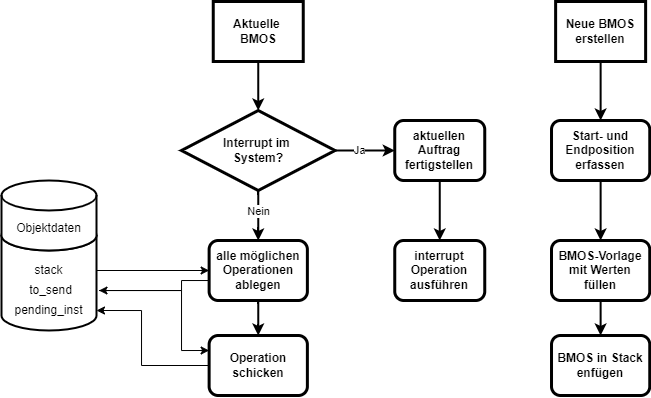
\includegraphics[width=0.7\textwidth]{stack.png}
    \caption{Diagramm der BMOS bereitstellung}
\end{figure}

Die Auftrage sind im Einkaufswagen o.ä. im Format 'Location -\> Location' hinterlegt. Um dies in eine Opeation zu zerlegen die die SPS versteht, wird eine Box-Moveing-Operation erstellt. Diese enthält alle Teilschritte, wie Schlittenposition oder Fördebandstracke, um eine Box von Position A zu Position B zu bringen. 
Die BMO wird dann in die einzelnen verwendeten Module, Förderband oder Lager, aufgeteilt und dann dem 'stack' zugeführt. Diese Instruktion enthält Daten wie:
\begin{itemize}
    \item 'instruction\_id': Eine fortlaufende Nummer um jede Anweisung zu identifizieren
    \item 'order\_id': Zusammenhängende Anweisungen, bzw. Anweisungen für die gleiche Box, haben eine gleiche Nummer
    \item 'relation': eine Liste mit 'instruction\_id's', welch vor dieser Anweisung erfüllt sein müssen
\end{itemize} 

Bei Auswahl der zu schickenden Anweisung, wird zuerst die aktuell von der SPS gemachte Anweisung vermerkt, danach weird in allen Modulen des 'stacks' nachgeschaut, welche Anweisungen jetzt ausgeführt werden können. Zu diesem Zweck wird die 'relation' einer Anweisung mit den bereits gemachten Anweisungen verglichen, wenn bereits alle relevanten Anweisungen gemacht wurden, wird der Auftrag in 'to\_send' vermerkt. Schlussendlich wird einer der in 'to\_send' vermerkten Aufträge für die SPS übersetzt und an diese geschickt. 
Wenn die SPS den Auftrag erhalten hat, schickt sie ein 'acknowledge' mit der erhaltenen ID zurück. Der Auftrag wird dann aus den 'instructions\_to\_send' gelöscht und entweder wird einfach der nächste Auftrag in 'to\_send' geschickt oder der 'BMOS' Algorithmus wird erneut durchlaufen.


\subsubsection{Datenbanken}

Als Datenbanksystem wird aufgrund des guten Supports MySQL gewählt. Dies ist ein relationales Datenbankmanagementsystem welches in einem Docker-Container aufgesetzt wird. In diesem werden alle Daten gespeichert, die zur Auswahl sowie zur Ausliferung von Teilen nötig sind.

\begin{figure}[h]
    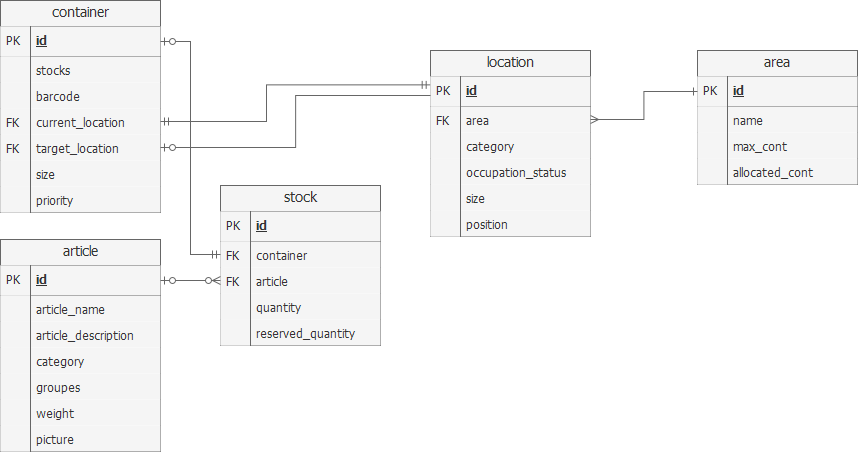
\includegraphics[width=0.6\textwidth]{DB-Schema.png}
    \centering
    \caption{Datenbankschema des AFSS}
    \label{DB-Scema}
\end{figure}

Wie in \ref{DB-Scema} ersichtlich, beinhalt diese Datenbank fünf Tabellen. Diese hohe Komplexität resultiert daraus, dass diese Struktur eine 100\%ige Flexibilität in der Ablage von Bauteilen in einem überliegendem System bietet.

Die Erste Tabelle beschreibt ein einziges theoretisches Bauteil. Dieses hat einen Namen, Gewicht, Beschreibung und Kategorien zur Filterung. Unter der Spalte 'picture' wird ein Dateiname gespeichert, der zu einem Bild zeigt, dass das Produkt abbildet.
Die zweite beschreibt einen Container. Im Lagersystem entspricht dieser einer Box. Diese kann mehrere `stocks' beinhalten, sowie durch einen Barcode identifiziert werden. Weiters muss jeder Container immer eine aktuelle Position (`current\_location') besitzen, an der die Box gerade ist. Im ausgelagerten (und noch nicht eingelagerten) Zustand ist diese `location' Position 0. Das Ziel der Box wird in `target\_location' gespeichert. Stimmt die aktuelle mit der Zielposition überein, so ist die Box an ihrem Ziel angelangt. Die Kategorie `size' beschreibt die Größe eines Containers und lässt somit theoretisch zu, dass in Zukunft auch unterschiedlich große Boxen zuverlässig in die richtigen Lagerplätze eingelagert werden. `priority' wird nicht verwendet.

Container und Artikel werden im sog. 'stock' verheiratet. Dieser kann als bauteilhaufen in einer Box verstanden werden. Es können also auch mehrere 'stocks' mit dem selben Container geben, dies würde mehreren verschiedenen Bauteilen in einem einzigen Copntainer entsprechen. Auch ist es möglich mehrere Container mit den selben 'stocks' abzubilden, welches ener aufteilung von Abuteilen auf mehrere Container entspräche.

Die Positionen der Container werden in Standorte ('locations') abgebildet. Diese entsprechen den Lagerplätzen. Sie sind einer darüberliegenden 'area' zugeordnet, welche einerseits einen Lagerschrank, aber weiters auch Module wie Vereinzelungsanalgen, abbilden kann. Standorte verfüghen weiters über eine Position welche in X, Y und Z-Richtung beschreibt, wo sich ein Standort im Referenzsystem des Lagers befindet. Auch die größe des Lagerplatzes wird abgebildet, um sicherzustellen, dass auf jeden fall nur die richtige Größe an Box eingelagert wird.


\subsubsection{Docker}


    Docker ist eine Umgebung, in der Softwareprojekte isoliert werden können. Da es besonders  bei Projekten mit viele Pakete, mit verschiedenen Versionen, zu konflikten kommen kann, ist es sehr hilfreich diese zu bündeln. \\
    Umgesetzt wird dies mithilfe von Containern welche einen gesamten Programmteil als alleinstehende Einheit enthält. Diese werden über ein 'Dockerfile' configuriert, welches sich im selben Ordner wie die Python-Anwendung befindet. In diesem werden Parameter wie die Python-Version und die benötigten pip-Pakete sowie den Programmeinstiegspunkt angegeben. \\ 
    Ein zweier Docker Conteianer wird mit einem MySQL-Image erstellt, dort wird die Datenbank aufgesetzt. \\
    Um diese zwei Container miteinander Kommunizieren zu lasen, ist es ntig ein sog. docker-compose.yml File zu erstellen. Dies enthält alle Informationen über verwendete container, deren Ports, sowie Speicher für Dateien (Volumes). Bei Testbetrieb wird der Datenbankcontainer aleinstehend bestrieben und mit einem anderen Port, keine Zugriffsprobleme zu generieren. In Produktion wird dann derselbe Container in den Containerverband übertragen und dort mit einem anderen Port weiterverwendet. \\
    Erstellt wird dieser Containerverband mit den Consolenbefehlt der auf das docker-compose File zugreift. 
    \begin{lstlisting}[language=bash]
        docker build docker-compose.yml\end{lstlisting}
    Dann werden auch alle Logs in der Kommandozeile ausgegeben. 


\subsubsection{Artikelsuche}
\paragraph{TF-IDF und Rust Implementierung} \hspace{0pt} \\
Der TF-IDF (Term Frequency-Inverse Document Frequency) Algorithmus, ist ein Weg um wichtige wörter aus Dokumenten zu extrahieren. Er wird verwendet um beispielsweise in Suchmaschienen, eine Suchanfrage mit Webpagecontent abzugleichen, und die am besten mit der Suchanfrage übereinsteimmenden Dokumente zu sortieren. \\
Im Fall dieser Anwendung werden die Daten aus der Artikeldatenbank als 'Dokumente'  angesehen und die Suchanfrage aus dem Suchfeld wird dafür verwendet um die am besten passenden Artikel zu finden.
\\
Durch den Relativ hohen Rechenaufwand bei dieser Suchoperation wird dieser in der Programmiersprache Rust implementert. Die Implementierung in Rust ist im vergleich zu Python schon bei relativ kleinen Datenmenge bis zu 5-mal schneller.

\subparagraph{Rust}\mbox{}\\
Rust ist eine sehr effiziente und schnelle Programmiersprache die in den späten 2000er und frühen 2010ern bei Mozilla und der Open-Source-Community entwickelt. Sie unterstützt unter anderem mehr Typensicherheit und verhindert viele Programmierfehler. (vgl. \cite{gpt_rust})

Die Funktion dieses Algorithmus ist in drei unterteile Unterteilt.

\begin{enumerate}
    \item Term Frequenz \\
    Die Termfrequenz gibt an, wie oft ein angegebenes Wort in einem Dokument vorhanen ist. Dies wird durch die Folgende Funktion kalkuliert.
    
    \begin{lstlisting}[language=Rust, caption={Berechnung der Termfrequenz}]
fn term_frequency(document: &str, term: &str) -> f64 {
    // Store the lowercase document as a String to ensure it lives long enough
    let lower_document = document.to_lowercase(); 

    // Split the document into words
    let normalize_document: Vec<&str> = lower_document.split_whitespace().collect();
    // Make sure the searchterm is lowercase
    let normalize_term = term.to_lowercase();

    // Count occurrences of the term in the document
    let count = normalize_document
        .iter()
        .filter(|&&word| word == normalize_term) // Compare each word with the term
        .count();

    // Calculate the term frequency as occurrences / total number of words
    let total_words = normalize_document.len();
    if total_words == 0 {
        0.0 // Avoid division by zero if the document is empty
    } else {
        count as f64 / total_words as f64
    }
}\end{lstlisting}

    Mithilfe dieser wird eine Liste aller Wörter und der Vorkommenshäufigkeit dieser erstellt.

    \item Die zweite Komponente ist dann die Inverse Dokument Frequenz. Diese gewichtet, die Anzahl der Dokumente in dem das gesuchte Wort enthalten ist relativ zur Gesamtdokumentanzahl vorkommt. Häufig vorkommende Worte wie z.B. 'und' werden hierbei weniger gewichtet als einzigartige Wörter.

\begin{lstlisting}[language=Rust, caption={Berechnung der Inversen Dokumentenfrequenz}]
fn inverse_document_frequency(term: &str, all_documents: &Vec<String>) -> f64 {
    let mut num_documents_with_this_term = 0;

    // Iterate over all documents to check if they contain the term
    for doc in all_documents {
        // Normalize both term and document by converting them to lowercase
        let lower_doc = doc.to_lowercase();
        let normalized_doc: Vec<&str> = lower_doc.split_whitespace().collect();

        // Check if the term exists in the document
        if normalized_doc.contains(&term.to_lowercase().as_str()) {
            num_documents_with_this_term += 1;
        }
    }

    // Calculate IDF
    if num_documents_with_this_term > 0 {
        // Apply the IDF formula: 1 + log(total_documents / documents_with_term)
        1.0 + ((all_documents.len() as f64) / (num_documents_with_this_term as f64)).ln()
    } else {
        // If the term is not found in any document, return 1.0
        1.0
    }
}
\end{lstlisting}
     \item Nun liegt Liste davon vor, wie oft ein Wort in den Suchdaten vorkommt, als auch, wie oft ein Suchbegriff in einem bestimmten Dokument ist. \\ Als nächsten Schritt werden diese beiden Werte für jeden Suchbegriff miteinander multipliziert und ergeben somit einen Vektor der die Suchwörter in Relation zu jedem einzelnen Dokument stellt.
    \item Als letzten Schritt wird der zuvor errechnete Dokumentenvektor (der IDF jedes Suchterms in jedem Dokument) mit dem Suchvektor verglichen. Die geschieht mit der sog. Kosinus-Ähnlichkeit.
    \begin{lstlisting}[language=Rust, caption={Berechnung der Cosinusähnlichkeit}]
fn cos_similarity(query_p: Vec<f64>, document_p: Vec<f64>) -> f64 {
    // Ensure that both vectors have the same length
    if query_p.len() != document_p.len() {
        return -1.0;
    }

    let mut dot_product = 0.0;
    let mut abs_doc_squared = 0.0;
    let mut abs_query_squared = 0.0;

    // Calculate the dot product and the magnitudes (squared)
    for i in 0..query_p.len() {
        dot_product += query_p[i] * document_p[i];
        abs_doc_squared += document_p[i].powi(2); // document_p[x] ** 2
        abs_query_squared += query_p[i].powi(2); // query_p[x] ** 2
    }

    // Calculate the magnitudes
    let abs_doc = abs_doc_squared.sqrt();
    let abs_query = abs_query_squared.sqrt();

    // Handle division by zero in case of zero vectors
    if abs_doc == 0.0 || abs_query == 0.0 {
        return 0.0;
    }

    // Return the cosine similarity
    return dot_product / (abs_doc * abs_query);
}\end{lstlisting}
    Nach der Berechnung dieser für jedes Dokument werden alle Dokumente sortiert und ja nach anforderung die benötigte Anzahl ausgegeben.
\end{enumerate}

Das Aufraufen der Rust-Funtionen von Python aus, ist nicht nativ unterstützt. Die einbindung erfolgt millels PyO3/maturin.

\subparagraph{Artikelsuche nach Kategorien}\mbox{}\\
Um auch einen simpleren Weg der Artikelfindung zur Verfügung zu stellen, wird außerdem die Möglichkeit implementiert, Artikel anhand von Attributen zu suchen. Zu diesem Zweck werden schon bei der Artikelerstellung Attribute für die Einträge \textit{Gruppen} und \textit{Kategorien} vergeben. In \textit{Gruppen} wird eine Art Pfad angelegt, der die Suche eingrenzt. Beispielsweise würde so ein Eintrag folgende Daten enthalten: \texttt{['Item', 'Verbindungssatz']}. So kann bei der Artikelsuche zuerst die Überkategorie \texttt{'Item'} und dann die Unterkategorie \texttt{'Verbindungssatz'} aus mehreren verschiedenen ausgewählt werden. Um Bauteile weiter zu unterscheiden, da es z. B. viele verschiedene Widerstände gibt, werden unter \textit{Kategorien} Einzelheiten zum Produkt, wie Wert, Farbe o. Ä., gespeichert.\\  
Diese Informationen werden auch vom TF-IDF verwendet, dienen aber spezieller dazu, möglichst sicher das gewünschte Bauteil in einem Durchklickmenü zu finden.


\subsubsection{Fazit}
Die serverseitige Software des AFSS, also das WMS und die Benutzeroberfläche, wurde im Laufe des Projekts sehr komplex. Dadurch war es eine sehr gute Entscheidung, den Server in einer Hochsprache auszuführen.
Um einen zuverlässigen Dauerbetrieb zu gewährleisten, wäre es jedoch noch nötig, Unittests für wichtige Funktionen wie APIs oder den Lageralgorithmus zu implementieren. Weiterhin müsste die Benutzeroberfläche noch benutzerfreundlicher gestaltet werden, da sie momentan noch eher rudimentär ausgeführt ist. Außerdem wären noch kleinere 'Quality-of-Life'-Änderungen durchzuführen. Insgesamt ist die Software aber bereits sehr ausgereift und kann die Anforderungen der Lagersteuerung und -verwaltung erfüllen.


